%
% PROJECT: <ETD> Electronic Thesis
%   TITLE: Looks Good to Me (LGTM): Authentication for Augmented Reality
%  AUTHOR: Ethan Gaebel
% SAVE AS: thesis-draft.tex
% 

\documentclass[12pt]{report}
%\documentclass[12pt,dvips]{report} -- ORIGINAL

\usepackage{hyperref}
\usepackage{graphicx}
\usepackage{graphics}
\usepackage{amsmath,amssymb}
\usepackage{mathtools}
\usepackage{caption}
\usepackage{subcaption}

\setlength{\textwidth}{6.5in}
\setlength{\textheight}{8.5in}
\setlength{\evensidemargin}{0in}
\setlength{\oddsidemargin}{0in}
\setlength{\topmargin}{0in}

\setlength{\parindent}{0pt}
\setlength{\parskip}{0.1in}

% Uncomment for double-spaced document.
%\renewcommand{\baselinestretch}{2}
\renewcommand{\baselinestretch}{1.75}

% \usepackage{epsf}


\begin{document}

\thispagestyle{empty}
\pagenumbering{roman}
\begin{center}

% TITLE
{\Large 
Looks Good to Me: 
Authentication for Augmented Reality
}

\vfill

Ethan D. Gaebel

\vfill

Thesis submitted to the Faculty of the \\
Virginia Polytechnic Institute and State University \\
in partial fulfillment of the requirements for the degree of

\vfill

Master of Science \\
in \\
Computer Science and Applications

\vfill

Wenjing Lou, Committee Chair \\
Ing-Ray Chen \\
Guoqiang Yu 

\vfill

April 25, 2016 \\
Falls Church, Virginia

\vfill

Keywords: augmented reality, device pairing, hololens, meta, holograms, sharing, authentication
\\
Copyright 2016, Ethan D. Gaebel

\end{center}

\pagebreak

\thispagestyle{empty}
\begin{center}

{\large Looks Good to Me: 
Authentication for Augmented Reality}

\vfill

Ethan D. Gaebel

\vfill

(ABSTRACT)

%Augmented reality is a powerful new computer interface paradigm that is going to reshape how people interact with computers. The diverse hardware on typical augmented reality headsets presents an opportunity to the security community to re-make how authentication is carried out, making it more usable for the everyday user and moving authentication away from the cloud and back to face-to-face interactions (when users are face-to-face anyway). In this paper we explore an authentication protocol to be used when users are face-to-face and have augmented reality headsets. This protocol uses the same idea behind how humans identify speakers: localizing a wave and comparing its location to a face's location, except here we deal with radio waves instead of sound waves. This protocol is designed to minimize the work required by the user, thus increasing the likelihood that it will be used and decreasing the likelihood of user error. We provide an implementation of the protocol as well.

Augmented reality is poised to become the next dominant computing paradigm over the course of the next decade. With three-dimensional graphics and interactive interfaces that rival the best science fiction novels. Users will want to have shared experiences in these rich mixed reality scenarios, but surely users will want to restrict who can see their content in certain scenarios. It is currently unclear how users of such devices will authenticate one another, particularly in scenarios where access to the Internet is restricted or undesirable. Traditional authentication protocols rely on a trusted authority to bootstrap authentication between two users, but augmented reality content sharing will usually occur in face-to-face scenarios where it will be advantageous to keep communications and authentication localized. Looks Good To Me (LGTM) is an authentication protocol for augmented reality headsets that leverages the unique hardware and context provided with augmented reality headsets to solve an old problem in a more usable and more secure way. LGTM works over point to point wireless communications so users can authenticate each other in any circumstance and is designed with usability at its core, requiring users to perform only two actions: one to initiate and one to confirm. LGTM allows users to intuitively authenticate one another, seemingly only each other's faces. Under the hood LGTM uses a combination of facial recognition and wireless localization to ensure secure ridiculously simple authentication.

\vfill

\end{center}

Security-based abstract and stuff!!!

\vfill

% GRANT INFORMATION
This work was supported in part by the National Science Foundation under Grants 
CNS-1443889, CNS-1405747, CNS-1446478, and CNS-1343222.

\pagebreak

% Dedication and Acknowledgments are both optional
% \chapter*{Dedication}
% \chapter*{Acknowledgments}

\tableofcontents
\pagebreak

\listoffigures
\pagebreak

\listoftables
\pagebreak

\pagenumbering{arabic}
\pagestyle{myheadings}

%%%%%%%%%%%%%%%%%

\chapter{Introduction}
Augmented reality is one of the most exciting new technologies on the horizon, promising three-dimensional interfaces that one or more users can directly interact with. These immersive interfaces are commonly provided via head-mounted displays with translucent lenses that render digital content in two or three dimensions on top of the real world. Many of these head-mounted displays will be stand-alone computers equipped with powerful processors, wireless communications, one or more high resolution cameras, and depth sensors. This sophisticated array of hardware is used to provide fully interactive augmented reality which requires: hand tracking, graphics processing, and wireless communication, since connectivity is a requirement for any consumer device today. \par

Users of augmented reality headsets have the same need that users of any other consumer electronic device have today: the need to send content to others. With augmented reality, this content will usually be far richer, and thus larger, than we've seen on other platforms, since users will be creating, viewing, and working with three-dimensional objects, which inherently have more information associated with them than their equivalent two-dimensional representations. It is also expected that users will share a large amount of content face-to-face since this will provide 3D objects that both users can see and/or interact with in real time. The current analog to face-to-face digital sharing in augmented reality is using a smart phone to show a video or picture to someone. The sharing action is the same, but the sharing medium has switched from physically displaying one's screen to another to sharing the content across two users screens. I expect this type of sharing to increase with augmented reality as much of the physical world's in person content exchanges transition to the digital world, like so many other content streams in the past. \par

Content sharing between users in close proximity is an interesting and well-studied problem \cite{TalkingToStrangersSmetters2002,P2pMobileSocialContentSharingQureshi2010,CarTorrentLee2007,P2pFileSharingMobileAdHocKlemm2003,VanetcodeVehicularNetworkCodingShabbir2006,CodeTorrentVanetLee2006,AdHocSharingSystemPatentVan2006}. In comparison, today's typical content sharing schemes take advantage of preexisting infrastructure such as cell towers, wireless access points, and the Internet. This makes sense considering the most common use case for digitally sharing content currently is to share it with those who aren't present. You wouldn't send someone standing next to you a video, you'd pull out your phone and show them. But with augmented reality you would send someone sitting next to you a video so that the two of you can watch it together through your respective headsets. \par

This type of local sharing deserves separate consideration from the general content sharing problem. As local sharing becomes more common it will be worthwhile to explore and design for the specific conditions that separate local sharing from remote sharing. One of the new augmented reality headsets to hit the market, the Microsoft HoloLens, recognizes the value in this and has separate support for local sharing vs. remote sharing \cite{HoloLensSharingLocalNetwork2016}. Local sharing is piped over a local area network instead of going through the Internet and back. Another way is with point to point wireless communication, which is a very small step from a local area network since most WiFi hardware can use WiFi Direct, a popular point to point wireless protocol \cite{WiFiDirectP2p2014}. Also, point to point wireless communication is more dynamic and universally usable since it doesn't require any infrastructure. \par

Regardless of how it is accomplished, local network resources should be used over global ones for local content sharing, particularly when the content is stored locally on a user's device, as will often be the case with photographs, three-dimensional scene captures, videos, shared app interfaces, and user-created three-dimensional content. By sharing content locally, network resources are saved and money may be saved if charge-by-data usage plans are being used for Internet access. On top of this, local content sharing is robust in the face of global infrastructure failures, and content sharing privacy details are kept between the two users doing the sharing instead of being shared with whatever entity is providing the sharing service, such as who is communicating with whom, what is being communicated, and when the communication is occurring. Our work in this paper focuses on specifically using point to point communication to facilitate local content sharing in augmented reality systems. This is largely to preserve generality, since point to point communication does not have any infrastructure dependencies. As a result of this generality, much of our work can be translated into the local area network approach to local content sharing. \par

% Begin exposition on my problem
When working in a localized communications scenario where there is no central authority, authentication can be tricky. It will often be the case that two users have not used their devices to communicate before, meaning there will be no preexisting security context between the two devices such as a pin, key, token, etc. This problem is commonly known as device pairing and it is well studied \cite{ConferenceCompStudySecurePairingKumar2009,VisualChannelPairingSaxena2006,InBandPairingGollaktoa2011,DucklingStajano2000,PlayfulPairingGallego2011,SASVaudenay2005,ManaGehrmann2004,ShakeWellBeforeUseMayrhofer2009,SeeingIsBelievingMcCune2005,TalkingToStrangersSmetters2002,LoudAndClearGoodrich2006,HapadepSoriente2008}. We go into more detail about existing device pairing work in the background section. \par 

Using our specific instance of device pairing, we have developed a novel solution to pair two augmented reality headsets that is quick and simple while providing a high degree of security. This solution leverages the unique hardware capabilities required for augmented reality along with facial recognition and very recent advances in the area of wireless localization. The core idea of our scheme relates to how humans authenticate other human speakers. When trying to determine whom is speaking, our brains localize the source of the audio signal heard and then we match up that origin with a face that our brain has also recognized \cite{SoundLocalizationHumanListenersMiddlebrooks1991,FaceVoicePersonPerceptionCampanella2016}. Humans take a wave-signal source, localize it, then pair it with a face. Our work builds on this idea except instead of localizing an audio signal we localize a wireless signal that is adjacent to a face and recognize the face automatically using facial recognition. By doing this, we create an authentication scheme robust against man-in-the-middle attacks that reduces the problem of pairing for the user to simply looking at another user's face and indicating to their augmented reality headset that it ``Looks Good To Me'', thus establishing a secure connection. This system is aptly called ``Looks Good To Me'' or LGTM for short. \par

In this paper we present the two-party device pairing protocol LGTM along with a full open-source implementation of the protocol. The remainder of this paper is divided up as follows. Section II surveys several relevant areas including augmented reality and device pairing. Section III presents the system model, threat model, security objectives, and the LGTM protocol. Section IV presents analyses of LGTM covering security, usability, and privacy implications of LGTM. In section V we present the details of our implementation of LGTM, including a link to the complete open-source code-base. Section VI presents experimental results involving localization accuracy and overall protocol performance. In section VII we discuss research areas that could improve LGTM further. In section VIII we conclude. \par


\section{Background}
\subsection{Augmented Reality}
Augmented reality has been around as a research topic since as early as 1993 \cite{RealWorldArWellnet1993}, but only recently have augmented reality headsets been pursued as consumer and business products \cite{MagicLeapWebsite,MetaWebsite,HoloLensWebsite,GoogleGlassWebsite}. Augmented reality at its core is taking what we see in reality and overlaying additional digital objects on top of reality in the form of two-dimensional or three-dimensional renderings. Additionally, users can directly interact with the digital objects using their hands or other parts of their body. Additional peripheral devices may be used to increase immersion and responsiveness, but the most common case is for users to use their hands. \par

There are several different ways to render digital objects over reality. Augmented reality smart phone apps exist on every platform and these apps rely on taking in reality from the smart phone's camera and other sensors, displaying it on the smart phone screen, and rendering additional digital objects over reality on the screen of the smart phone \cite{LayarArApp,GoogleTranslate,IonRoadArApp}. More natural approaches to augmented reality rely on projectors, some of which require special glasses to view properly \cite{VtCubeWebsite}. However the vision for future augmented reality experiences lies in the head-mounted display, a large pair of glasses with a mechanism to deliver light encoding specific digital objects directly into the user's field of vision. The first such head-mounted display to gain public notoriety was Google Glass \cite{GoogleGlassWebsite}. Glass renders two-dimensional objects into the user's field of vision and really acted as an ever-present extension of the smart phone interface. This interface was used via voice commands and buttons on the side of the glasses. This version of Glass did not become a consumer product and indeed it may have partially sullied the reputation of augmented reality. Now however we see a wave of augmented reality head-mounted displays coming to market. The Meta 1 and 2 \cite{MetaWebsite} the Microsoft HoloLens \cite{HoloLensWebsite}, Magic Leap \cite{MagicLeapWebsite}, several small startups focused on augmented reality, and recent confirmation of Google working on a next generation of Glass \cite{WiredGoogleGlassNextGen2015}. A common characteristic of these new headsets is that they are more immersive than Glass, all allowing users to directly interact with digital objects using natural hand movements, enabled by infrared depth sensors that capture user gestures and the environment around them. Depth information is combined with other sensory data to provide a service referred to as SLAM, Simultaneous Location and Mapping \cite{ParallelTrackingAndMappingKlein2007,MonoSlamDavison2007,VisualIntertialOdometryNonlinearLeutenegger2014,ProjectTangoWebsite,SlamPart1Durrant-Whyte2006}. This current and upcoming augmented reality platform is the target platform for LGTM. \par

Another trend we see in practical augmented reality headsets is toward them being stand-alone computers. The Microsoft HoloLens is already a fully functioning computer, and the company Meta has stated that it intends to move toward a full stand-alone computer headset for consumer devices \cite{MetaWebsite}. This trend implies that augmented reality users will be able to enjoy all the current advantages of computers with the addition of the powerful sensors and paradigm changing user interfaces that come with augmented reality. This allows us to look at traditional problems that arise in the context of computers and computing and reexamine these existing problems and their existing solutions in the context of augmented reality computers with an eye to improve upon the current state-of-the-art by using the additional functionality provided via the hardware and abilities from augmented reality. One of these problems is device pairing, which is a common procedure that must be done to connect two devices together such as a headset and a smart phone, a speaker and a smart phone, two smart phones, or any other wireless peripheral with a smart phone or computer. \par

\subsection{Device Pairing}
Device pairing is the area dedicated to authenticating devices without prior security context, and there have been many schemes introduced to address this problem on devices with myriad hardware features and constraints \cite{PlayfulPairingGallego2011,BedaSoriente2007,ShakeWellBeforeUseMayrhofer2009,SeeingIsBelievingMcCune2005,TalkingToStrangersSmetters2002,LoudAndClearGoodrich2006,HapadepSoriente2008,VisualChannelPairingSaxena2006}. Virtually all of these methods rely on communication over one or more out-of-band channels. An out-of-band channel is any channel which is not the primary communications channel being used. This secondary channel can be defined quite broadly and many schemes use human sensory capabilities or human activity as the out-of-band channel. The primary channel that the secondary channel is used to authenticate is a human imperceptible channel, most often the wireless channel. So most device pairing schemes proceed as follows. Some information is transmitted over the out-of-band channel, which is then used for authentication in the primary channel via some specialized authentication procedure. These authentication procedures can vary widely depending on what sort of out-of-band channel is used and what sort of information is transmitted across it. The simplest and most common example is for a numerical pin to be exchanged or verified between two devices via one or more human actors. Depending on the scheme, the pin may need to be entered on both devices, transmitted between two devices and then verified as matching by one or more users, or some complex combination of the two \cite{Bluetooth40Spec2010,BluetoothInterfaceFlowSecureSimplePairing2007,JournalCompStudySecurePairingKumar2009}. When human actors are involved, the exchanged information is often short to improve usability \cite{BluetoothInterfaceFlowSecureSimplePairing2007}, and thus possesses a low level of entropy, reducing its security. As a result, a good deal of research has gone into how to improve the security short strings. The two dominant protocols that have emerged from this are known as short authenticated string (SAS) protocols \cite{SASVaudenay2005} and so-called manual authentication (MANA) protocols \cite{ManaGehrmann2004}, with SAS protocols enjoying more widespread use in practical systems such as Bluetooth \cite{Bluetooth40Spec2010}. \par

Bluetooth versions 2.1 and beyond use secure simple pairing for pairing two devices and it includes four different pairing options \cite{Bluetooth40Spec2010,SimplePairingAnalysisBluetooth4Phan2010,FormalAuthAnalysisBluetoothChang2007}: (1) numeric comparison, where both devices display a 6-digit numeric string that must be confirmed on both devices; (2) passkey entry, where the user enters a 6-digit numeric string on one or both devices, in the case where the 6-digit numeric string is entered on one device it must be verified on the other; (3) out-of-band mode, where a secure key is agreed upon using a non-human out-of-band channel, such as near-field communication (NFC); and (4) just works, which unlike the other three options, does not have any protection against man-in-the-middle attacks. Just works prompts the user to confirm a device name that does not have security properties; the only security provided in just works mode is through timing and Bluetooth's relatively short range, neither of which protects a user from a determined attacker in a public space. Just works was included for compatibility and usability reasons, to maintain compatibility with Bluetooth 2.0 devices, and to improve usability for end users \cite{BluetoothInterfaceFlowSecureSimplePairing2007} if they decide that the other three techniques are too much of a hassle. It should come as no surprise that the just works option has become a primary attack point on the secure simple pairing protocol \cite{BluetoothSSPAttackJustWorksHaataja2008}. This security compromise for usability and backwards compatibility, which is really another sort of usability, has opened up a multitude of devices to attack. But usability is central to device pairing since human interaction is almost always a requisite component for bootstrapping authentication between two devices that have no preexisting context. \par

Usability in device pairing schemes has accumulated its own body of research \cite{UsabilitySecurityOutOfBandPairingKainda2009,UserPerceptionPairing,PlayfulPairingGallego2011,AliceMeetsBobKumar2009,SecurePairingUsabilityUzun2007,ConferenceCompStudySecurePairingKumar2009} through protocol comparisons, usability studies, and analyses of security issues that usability can affect. Usability is important because it can affect protocol adoption and even the security of the the protocol. If users are prompted to confirm a numeric string that appears on a pair of devices, and they confirm it without thorough checking, it is easy for incorrect devices to be authenticated, which is a huge security leak. One study investigating usability's impact on security in device pairing protocols found that users made mistakes with 4-digit numeric comparison-based pairing that lead to security errors 20\% of the time \cite{SecurePairingUsabilityUzun2007}. The study found security errors to be alarmingly high for three other pairing schemes based on entering and comparing 4-digit numeric strings as well. The device pairing community has given a great deal of attention to inventing new pairing protocols which rely on new hardware capabilities \cite{PlayfulPairingGallego2011,BedaSoriente2007,ShakeWellBeforeUseMayrhofer2009,SeeingIsBelievingMcCune2005,TalkingToStrangersSmetters2002,LoudAndClearGoodrich2006,HapadepSoriente2008,VisualChannelPairingSaxena2006}, but many of these schemes have been found to not be very usable when given to users \cite{SecurePairingUsabilityUzun2007,ConferenceCompStudySecurePairingKumar2009}. This was further examined in \cite{UserPerceptionPairing}, where usability studies coupled with user interviews revealed that users prefer different pairing methods based on the context: location, time urgency, and sensitivity of the information being exchanged after pairing. The study also revealed that many non-technical users are interested in using new pairing techniques, but that their perceptions of security and the context in which the pairing was occurring greatly influenced which pairing technique was going to be used. \par

% ADd brief paragraph about AR & pairing with peripherals
Pairing using augmented reality headsets is a greatly unexplored subset of device pairing, which is understandable due to the newness of practical augmented reality headsets. However, it has recently been revealed that the Microsoft HoloLens can use QR codes that are displayed on a device, with either a screen or a sticker, to authenticate peripheral devices \cite{HoloLensVisualPairing2016}. Beyond this, we are unaware of any device pairing work having been done with augmented reality headsets, making our work on LGTM one of the first to specifically address pairing on augmented reality headsets. \par


\chapter{LGTM Protocol}
\section{Security Opportunities with Augmented Reality}
Device pairing schemes have taken advantage of myriad interesting sensors and hardware, but many of these have involved unrealistic or awkward pairing scenarios. With the paradigm shift that is augmented reality we have an influx of new hardware coupled with a new sort of user and device context that includes how certain pieces of hardware are positioned. For instance, on smart phones the main camera is positioned on the back of the phone and is generally not facing the same direction as the user's gaze. But with augmented reality the camera is lined up with the user's line of sight. This context can be leveraged in interesting ways. With this setup the augmented reality headset can preprocess what the user is seeing. This preprocessing can lead to the user's vision being annotated in certain ways that the user finds useful. Another example of hardware positioning that we can utilize is that of wireless communications antennas. Wireless localization can now be used for more than just localizing a device, thanks to the close proximity of the wireless antennas to a person's face, we can localize a wireless signal and then pair that location with a user's face using proximity alone. 

By combining the area occupied by a user's face with the area of a wireless signal's origin we can localize the signal, preprocess the area around the signal's origin by searching for a face matching some facial recognition model, and present matching faces to the user for verification, thus associating a specific user with a specific wireless signal and authenticating both. We can use this authentication to secure key exchange mechanisms, like Diffie-Hellman, from man-in-the-middle attacks and provide an incredibly usable device pairing experience to users. \par

Consider this scenario: Alice and Bob meet for the first time and want to pair their augmented reality headsets to exchange some three-dimensional content. Alice and Bob both trigger the pairing protocol on their devices. Moments later they are both prompted to confirm one-another's faces, which are outlined on their respective augmented reality displays. Alice and Bob confirm one-another's faces and now they are free to communicate over an encrypted channel. What could be simpler than that? This is what LGTM promises. \par

\section{System Model}
First we must adequately understand the scenarios where the Looks Good to Me (LGTM) authentication protocol is applicable. This requires us to go down the list of hardware requirements, security context, the users' context, and all other assumptions we make. 
LGTM is specifically designed for authenticating two users, Alice and Bob. Alice and Bob are assumed to be users equipped with head-mounted augmented reality displays which are also stand-alone computers equipped with: wireless communications hardware with support for a point to point communications protocol, software and hardware support for wireless localization using the same wireless hardware used for communication, a high-definition video camera, and a translucent display directly in front of the users' eyes that is capable of displaying digital objects on top of the physical world (this last requirement is satisfied simply by the users possessing head-mounted augmented reality rigs, but we want to be thorough). \par

The two hardware devices are assumed to have no prior security context, which means the two devices do not possess any information that can be used to prove the authenticity of their claimed identity to the other. A pre-shared key is a common example of a piece of information which can be used as preexisting security context. \par

An important piece of information that each headset is assumed to possess is a facial recognition model capable of recognizing the user of the headset. That is, Alice's headset has a facial recognition model that can recognize her, and Bob's headset has a facial recognition model that can recognize him. Training these models can easily be done in a mirror. \par

As for the users themselves, Alice and Bob are assumed to be in sight of each other and would like to share some sort of digital content with one another, such as a shared application experience, a shared video, shared music, shared holograms, or basic messaging. No assumptions are made of Alice and Bob's relationship with each other: they may be friends, acquaintances, or strangers. \par

No assumption regarding access to the Internet is made. \par

\section{Security Objectives}
% (Security) Objectives
% ---- Authenticate the wireless signal of one user so that secure 
%           communication can be done between two individuals
% -------- Bootstrapping authentication
% ---- Select a user-wireless signal pair to communicate with
% -------- Selection problem
% ---- Privacy Objectives (sub-section under security objectives...)
% -------- No need for centralized power knowing communication/content patterns
% -------- Intermediary parties facilitating communication is 0
% ------------ The potential for remote eavesdropping, censorship, tracking, 
%                   etc, is non-existent
The primary security objective is for Alice and Bob to correctly authenticate one another's wireless signals so that they can engage in secure point to point wireless communication. Recall from the system model section that Alice and Bob do not share any security context, so this authentication must be bootstrapped. \par

A secondary objective is for Alice and Bob to correctly select which user they want to communicate with. This objective is directly related to the first but it warrants distinction as a worthy problem on its own merit since there are many practical attacks that rely upon tricking users into selecting the wrong thing \cite{PairingInterfaceConstrainedRushingSaxena2009,WhyPhishingWorksDhamija2006} and researchers have even begun examining this problem in augmented reality systems specifically \cite{SecurityAndPrivacyForARRoesner2014}. We refer to this as the user-selection problem. \par

\section{Threat Model}
% Threat Model
% ---- Wireless attacker model
Attackers have quite a bit of power when dealing with a wireless channel since the communications medium is both public and localized. Attackers have the capability to: jam communications, perform denial-of-service attacks by flooding the channel with packets constructed to fit the protocol, eavesdrop on all packets transmitted, and replay packets collected from eavesdropping in any order. Further, the attacker may have multiple transceivers at his or her disposal, so attacks can be coordinated between more than one node. However, it is necessary for an attacker to be physically present, either personally or via a device which he or she controls remotely. \par

Attackers may use these capabilities to accomplish one or several goals. An attacker may want to impersonate Alice to send Bob falsified content. An attacker may want to impersonate both Alice and Bob to perform a man-in-the-middle attack allowing the attacker to eavesdrop on encrypted communications between Alice and Bob. The attacker may simply want to prevent communication between Alice and Bob. Or the attacker may want to do any of the above steps with the higher goal of exploiting some subsystem. \par

\section{Protocol}
% Protocol, high level (high-level, as in the protocol diagram)
To begin the protocol, Alice presses a button which may be digitally rendered over reality or physically located on the augmented reality headset. At this point Alice's headset begins listening on the local wireless channel and broadcasts an initialization packet containing: Diffie-Hellman parameters $g$ and $p$ corresponding to a generator over a group and a prime number, respectively, Alice's Diffie-Hellman public key, and a randomly generated number. Since Bob is not listening yet, Alice's message goes unanswered. Bob presses a button to activate the protocol, opening his device up to listen to the wireless channel and generating an initialization packet containing Diffie-Hellman parameters $g$ and $p$, Bob's private key $b$, Bob's public key computed as: $B = g^b \: mod \: p$, and a randomly generated number, $R_{B1}$, to serve as half of a session identifier. Bob broadcasts his message $g || p || B || R_{B1}$. Alice receives Bob's initialization packet and generates her private key $a$ and computes her public key in relation to the received Diffie-Hellman parameters $g$ and $p$ as $A = g^a \: mod \: p$. Alice generates a random number $R_{A1}$, to serve as the second half of a session identifier and broadcasts her public key $A$ concatenated with the random number $R_{A1}$, and $R_{B1} \oplus R_{A1}$, which is the session identifier for Alice and Bob's current session, where $\oplus$ denotes the exclusive-or operation. This makes Alice's full message: $A || R_{A1} || (R_{A1} \oplus R_{B1})$. Bob receives Alice's message and verifies that it is in response to his initial message by checking that $R_{B1} \oplus R_{A1}$ equals the final number in Alice's message. Alice and Bob both compute the shared key $K = B^a \: mod \: p = A^b \: mod \: p$. At this point Alice and Bob have established a shared symmetric key, but have not established the authenticity of each other's identities. \par

Bob retrieves facial recognition parameters that define a facial recognition model to recognize his face, $F_{B}$. Bob encrypts the facial recognition parameters using the shared key and an initialization vector, IV, which Bob concatenates with his encrypted facial recognition parameters, $IV || E(IV, K, F_{B})$, and broadcasts this. Alice receives Bob's encrypted message with his facial recognition parameters and also records the channel state information, $CSI_{A}$, associated with the packets carrying Bob's message. Alice decrypts the message and retrieves $F_{B}$. Alice computes Bob's location using a wireless localization algorithm denoted by $G(\cdot)$ to get Bob's location: $L_{A} = G(CSI_{A})$. Alice runs a facial recognition algorithm denoted by $H(\cdot)$, using Bob's facial recognition parameters to obtain a location for any faces that match $F_{B}$, denoted by $FL_{A} = H(F_{B})$. Alice compares $L_{A}$ and $FL_{A}$ to see if the coordinates overlap. If they do not match then they are thrown out. If there are no matches among all the options for $L_{A}$ and $FL_{A}$ then the protocol is aborted. If there are matches, then Alice's device renders a box around Bob's face, matched by $F_{B}$, and whose location, $FL_{A}$, overlaps with the corresponding $L_{A}$. Alice is prompted to verify that the protocol has selected the correct face. In practice, there may be many pairs of faces and locations to check at once since multiple users may be carrying out LGTM at the same time. In this case Alice selects Bob's face from the available faces, if it is present. If Alice fails to select Bob's, face then the protocol aborts at this point. \par

Otherwise, Alice retrieves facial recognition parameters that define a facial recognition model to recognize her face, $F_{A}$. Alice uses the shared key, $K$ and the last several bytes of $F_{B}$ as an initialization vector, IV, to compute the encryption, $E(IV, K, F_{A})$ and broadcasts it. Bob receives Alice's encrypted message with her facial recognition parameters and also records the channel state information, $CSI_{B}$, associated with the packets carrying Alice's message. Bob decrypts the message using the shared key, $K$, and the initialization vector derived from the last several bytes of $F_{B}$ and retrieves $F_{A}$. \par

Bob computes Alice's location using the wireless localization algorithm to get: $L_{B} = G(CSI_{B})$. Bob runs the facial recognition algorithm, using Alice's facial recognition parameters to obtain a location for any faces that match $F_{A}$, denoted by $FL_{B} = H(F_{A})$. Bob compares $L_{B}$ and $FL_{B}$ to see if the coordinates overlap. If they do not match, then they are thrown out. If there are no matches among all the options for $L_{B}$ and $FL_{B}$, then the protocol is aborted. If there are matches, then Bob has a box drawn around Alice's face, matched by $F_{A}$, and whose location, $FL_{B}$, overlaps with the corresponding $L_{B}$. Bob is prompted to verify that the protocol has selected the correct face. In practice, there may be many pairs of faces and locations to check at once since multiple users may be carrying out LGTM at the same time. In this case Bob selects Alice's face from the available faces, if it is present. If Bob fails to select Alice's face then the protocol aborts. Otherwise, the protocol has successfully completed, Alice and Bob have established a secure key $K$, and they have authenticated each other's wireless signals ensuring that they are communicating with who they think they are. They are now free to send encrypted content back and forth. \par

\begin{figure}[!htb]
    \begin{center}
        \caption{Protocol diagram.}
        \label{figure: protocol-diagram}
        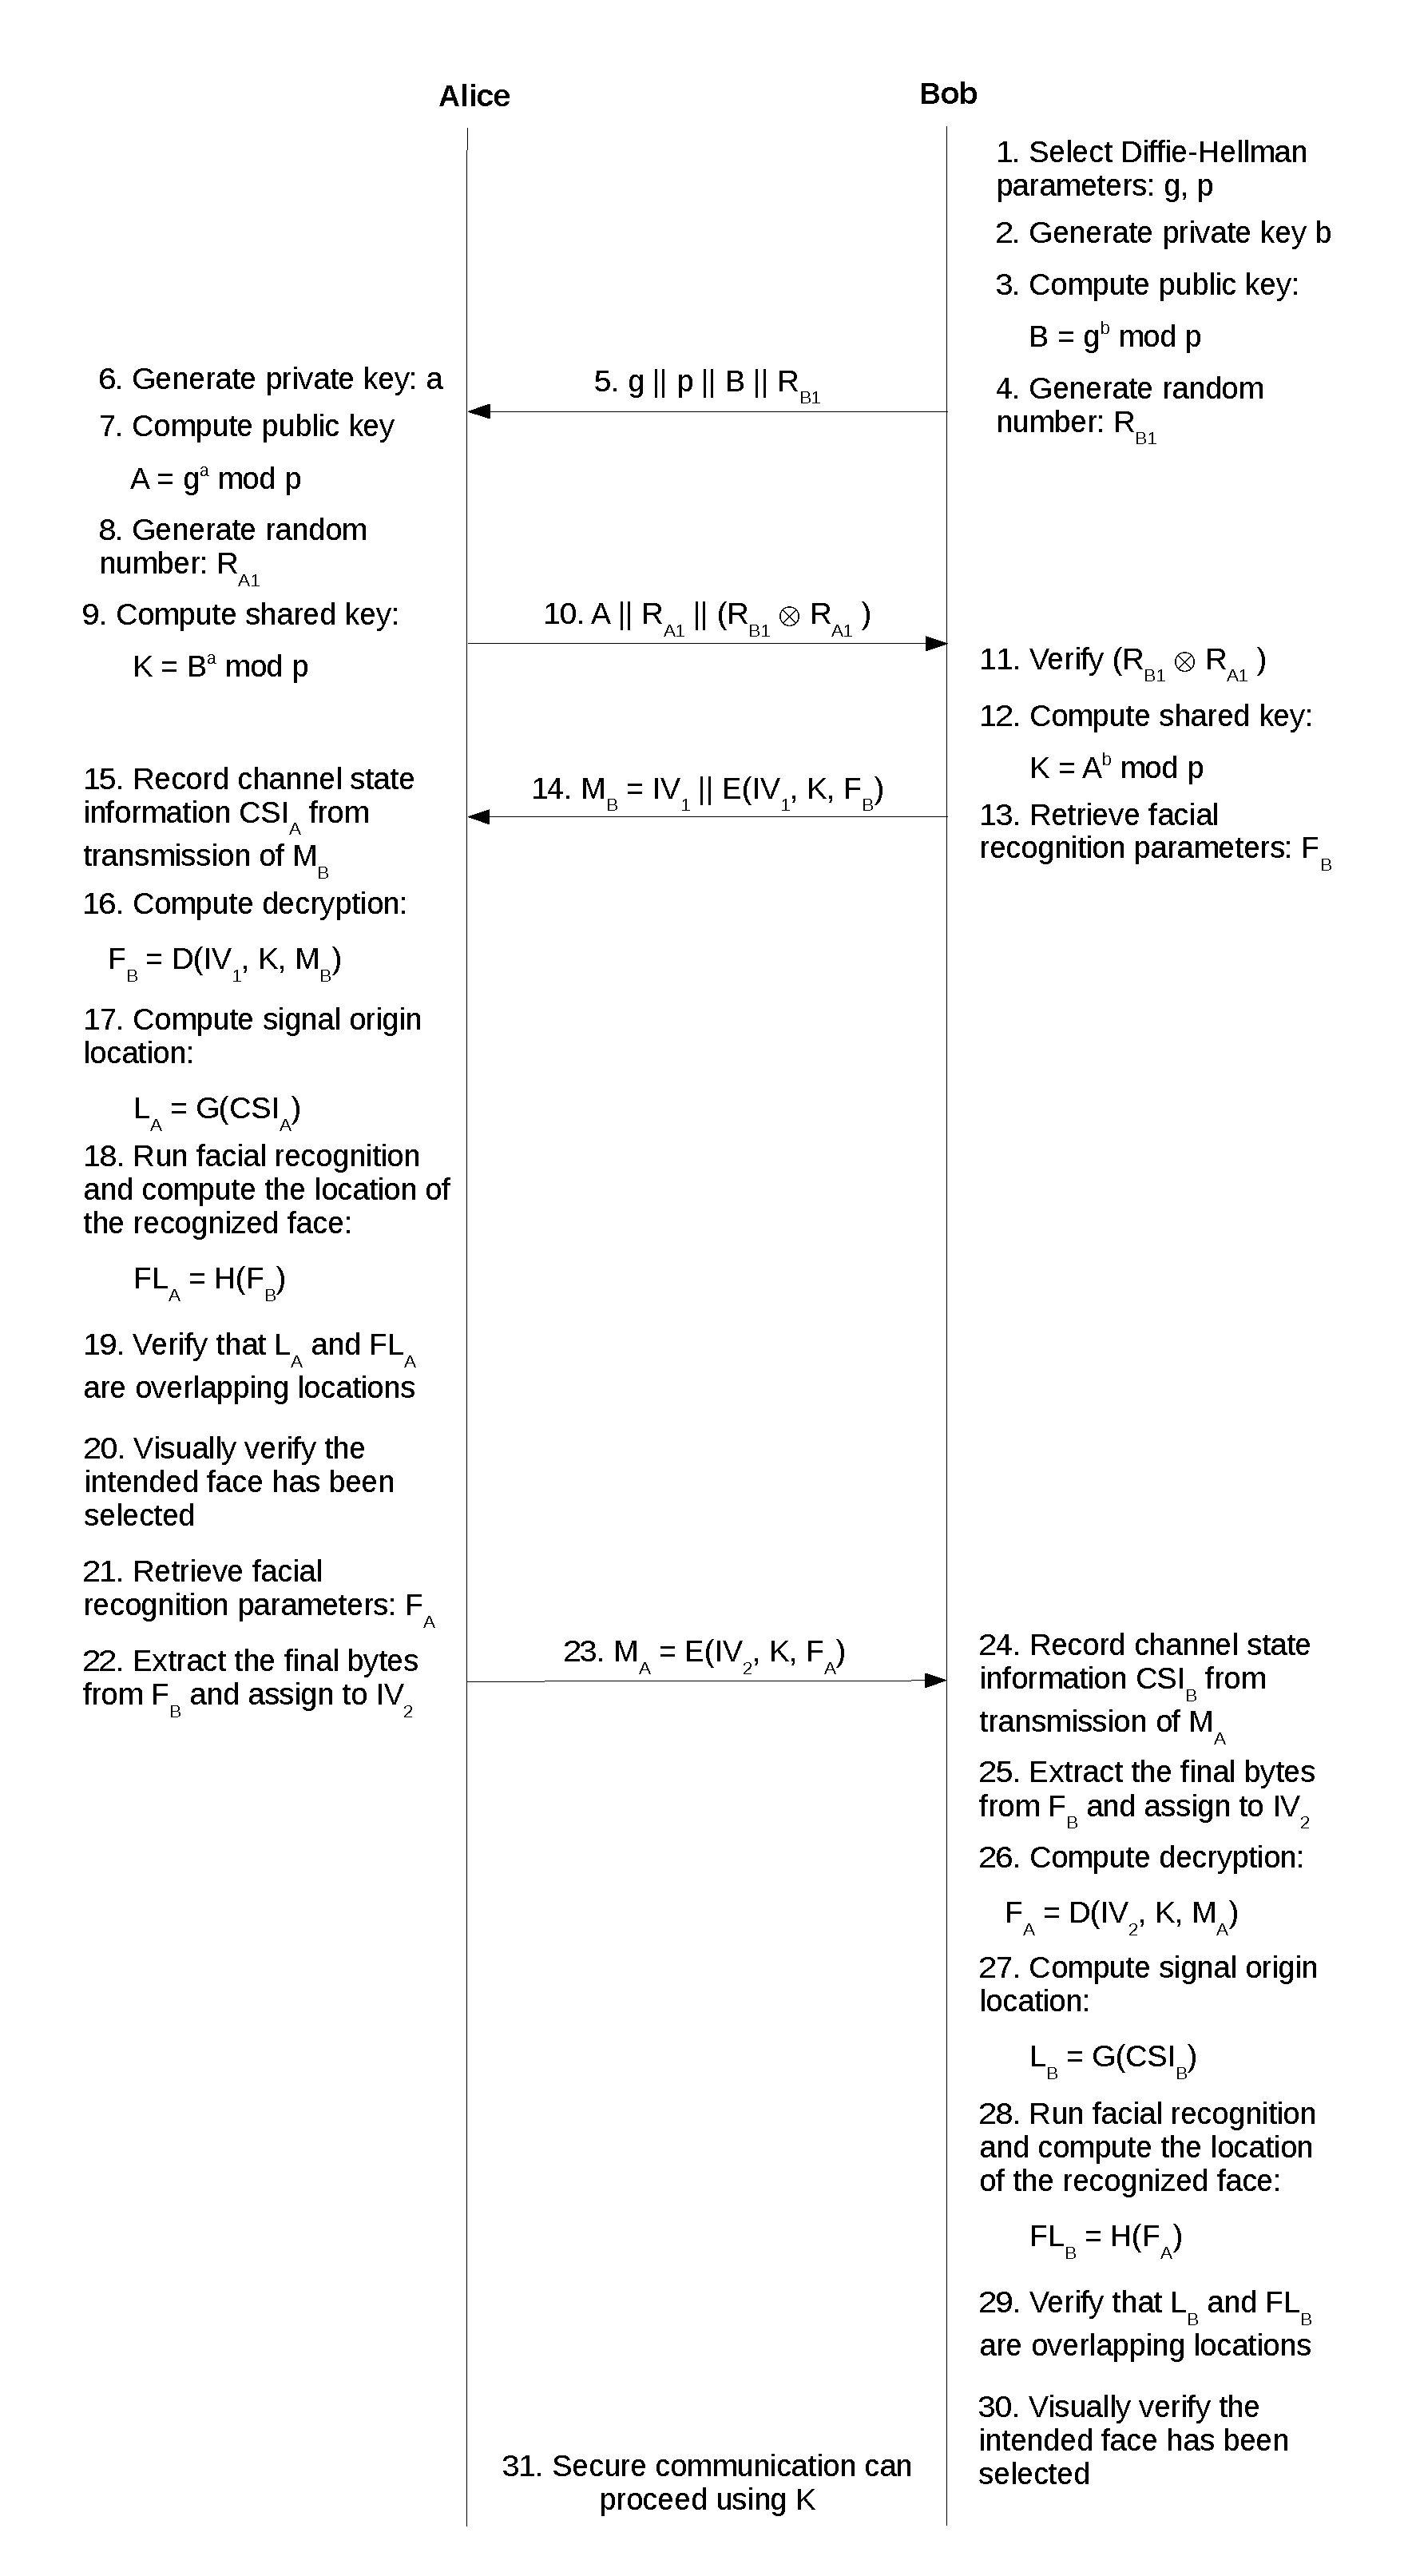
\includegraphics[scale=0.4]{../figures/looks-good-to-me-protocol-diagram.pdf}
    \end{center}
\end{figure}

\section{Protocol Analysis}
\subsection{Components (This title sucks, get a better one)}
% TODO: I need a grand intro that weaves together a story so that this section seems less like a list.... Perhaps I should put all the security guarantees that LGTM provides first, THEN explain how each one is achieved....
LGTM uses several techniques to achieve user authentication. As a result, it's constructive to unpack the purpose of each technique along with what LGTM gains by having that technique included. \par

LGTM uses Diffie-Hellman key exchange \cite{DiffieHellman2006} for establishing a shared key between Alice and Bob. Using Diffie-Hellman provides fast public-private key pair generation, even more so if elliptic curve Diffie-Hellman is used. High-speed key generation allows us to generate a new key pair every time we perform pairing. Making the public-private key pairs ephemeral provides LGTM with perfect forward secrecy, meaning that if an attacker obtains one of the private keys used in a single pairing the other public-private key pairs along with the symmetric keys derived from them remain secure. \par

In practice Alice and Bob may be receiving several messages at once since it is not apparent which wireless signals can be ignored and which one should be focused on until the protocol is complete. To differentiate between wireless signals, Alice and Bob use the random numbers, $R_{A1}$ and $R_{B1}$, and combine them using the exclusive-or operation to generate a unique session key. Using this session key, Alice and Bob can quickly determine which stream of messages an incoming message belongs to, but this session key does not have security guarantees; it is only used for message routing in non-malicious scenarios. \par

LGTM's security rests atop wireless localization's accuracy. Localization connects a wireless signal to a physical location by computing the signal's point of origin. This location can be matched with a device or person occupying that location, and with human assistance, this device or person can be authenticated. Wireless localization remains a difficult and unsolved problem and many current schemes are too inaccurate to be suitable for security applications. Very recent work has show great strides in improving localization precision and in reducing the amount and cost of hardware required to perform localization \cite{UbicarseKumar2014,SpotFiKotaru2015,ChronosSingleAPLocalizationVasisht2016}. The most recent and most promising of these methods \cite{ChronosSingleAPLocalizationVasisht2016} achieves a median error of 65 cm in line of sight conditions with a single laptop equipped with the Intel 5300 wireless card and three antennas. Consider now that LGTM's localization scenario is a constrained one. If two users are performing LGTM, they must have a line of sight between each other and in the most common use-case, they will be quite close to one another, likely within three meters. If we look at the results in \cite{ChronosSingleAPLocalizationVasisht2016} with these constraints in mind, we see that this localization technique achieves accurate localization down to less than 20 cm median error, which is sufficient for security applications. \par

This brings us to facial recognition. We state above that wireless localization is what allows LGTM to authenticate a device or person, so of what use is facial recognition? Having users authenticate a physical location, identified by say, a sphere, requires users to search for the sphere and verify that it intersects with the person they're attempting to communicate with. The facial recognition parameters exchanged in LGTM serve to make it easier for the user to solve the user-selection problem. Humans are phenomenal at facial recognition. It was found in \cite{NewbornsFaceRecognitionTurati2006} that infants as young as 1-3 days old are able to recognize faces. LGTM only asks for facial verification, not even full recognition. Verifying that an encircled face belongs to the person being authenticated is a far simpler task than verifying that a sphere intersects with the person's face. This is a great win for usability. In practice, users may be performing LGTM with several parties at once since they do not know which party is actually the one they wish to communicate with until the protocol is complete. This could result in several spheres being scattered across a user's vision, which may or may not match up with anyone's current location since the original source of the signal may have moved. By using facial recognition to effectively preprocess what the user is currently seeing, we are able to eliminate locations obtained via localization that do not match up with the location of the face identified by the facial recognition parameters. This reduces the chances of a user selecting an invalid location either accidentally or through an attacker's careful misdirection. Once the invalid selections are eliminated, there may still be multiple valid face-location pairs to choose from, but selecting a face remains a far simpler task than picking out a sphere or another sort of location representation. \par

Using facial recognition parameters to aid in the user-selection problem does not just affect usability, it also affects security. While the facial recognition parameters are not considered private, they are not instantly obtainable either. Training a facial recognition model for someone requires several photographs of that person, which can be obtained either online, by performing LGTM with the person, or in person by taking photos of the person. This is perfectly feasible for a targeted attacker, but this work in obtaining facial recognition parameters serves to significantly dampen the powers of spontaneous random attackers. \par

Consider a small node with wireless capabilities hidden in a discrete location that is designed to exploit every opportunity to attack wireless protocols. This node will be unable to attack LGTM since it would have to obtain facial recognition parameters as well. Furthermore, LGTM is specifically designed so that such a node cannot begin LGTM with a user and obtain their facial recognition parameters for use later. Notice in \ref{figure: protocol-diagram} the user who initiates LGTM sends his or her facial recognition parameters and is authenticated first, meaning a malicious user cannot use LGTM to harvest other users' facial recognition parameters without providing valid ones themselves, along with a valid human face that matches them. This makes the spontaneous random attacker's task significantly more difficult. \par

The final step in the protocol is for the actual human users to select a face from the options LGTM provides. As mentioned before, humans are excellent at identifying other human faces. On top of this, humans are great at recognizing the difference between a mask and a true human face. Without the human verification step, LGTM could be fooled by an attacker wearing a mask. Human verification serves as a final check against spoofing attempts. On top of this, as stated before, a user may be unintentionally performing LGTM in concert with several users at once. At the end of the protocol, the user may have several faces left to select from, and so the user must select one face from several potential choices, solving the user-selection problem. In most cases, the selections will be very limited since the two users are expected to be facing one another and to have a very short time window to initiate the protocol. \par


\subsection{Security Against Attacks}
We have spoken at length about the security properties the techniques used in LGTM possess; now we discuss how LGTM performs against attacks. \par

Man-in-the-middle attacks plague virtually every pairing protocol \cite{ConferenceCompStudySecurePairingKumar2009}. The very nature of pairing opens these protocols up to man-in-the-middle attacks since the purpose is to bootstrap authentication when there is no prior authentication information. This absence makes it possible for attackers to insert themselves in-between the two devices and trick them both. LGTM, however, has protection against man-in-the-middle attacks not afforded to other pairing protocols thanks to wireless localization. Localization pairs a signal to a location so attackers must occupy the same physical location as both users to successfully launch a man-in-the-middle attack. This is theoretically possible using two coordinated devices, although very difficult. \par

An attacker, Eve, can use two small devices physically attached to Alice and Bob's augmented reality headsets that mirror the messages between Alice and Bob, replacing the Diffie-Hellman public keys and random numbers with her own. These devices could forego localization since they do not have any way to verify the locations of Alice and Bob and pushing through the protocol, ``verifying'' every response they get. This will result in two nearly identical choices for Alice and Bob. This sort of man-in-the-middle attack can be mitigated by notifying the user that two devices appear to be occupying almost the same space. However, users often rush during authentication stages \cite{PairingInterfaceConstrainedRushingSaxena2009}, so users may complete LGTM before the second choice is presented, and it is unclear which device will be presented first. This entire attack procedure may sound rather preposterous, but as electronics shrink more and more, this attack will become more and more feasible. While not a large threat today, it may be a significant one in the future, perhaps even by the time augmented reality headsets become popular consumer products. \par

A more realistic man-in-the-middle attack for the present is one reliant on inaccurate localization results. As mentioned above, localization can not be called a solved problem yet, and any implementation of LGTM will have to deal with the currently accepted localization techniques, errors and all. The procedure would proceed as in the attack above, except Eve's devices will not need to be as close. We assume that implementors of LGTM will not rely on security through obscurity, so Eve will be aware of the localization abilities of Alice and Bob's device's implementations. Eve can position her devices behind, adjacent to, or in front of Alice and Bob with less precision and run her man-in-the-middle attack as above. \par

Inaccurate localization results can also be used in one-way impersonation as shown in \ref{figure: user-impersonation}. Eve might want to impersonate Alice to Bob, so she sets up a device near enough to Alice to fool the localization procedure and transmits Alice's facial recognition parameters. Eve will also need to obtain a facial recognition model for Alice, which she can do by participating in LGTM with Alice, searching for photos of Alice on the Internet, or by taking photos of Alice herself and then training a facial recognition model. As mentioned in the previous subsection, this attack will be partially defended against in the case where Eve is a spontaneous random attacker since the facial recognition parameters, while not secret, do take some work to acquire, work which an attacker is most likely unable to do if she is attacking random users. \par

\begin{figure}[!htb]
    \begin{center}
        \caption{Eve performs a user-impersonation attack by broadcasting from behind Bob, thus impersonating Bob to Alice.}
        \label{figure: user-impersonation}
        \centerline{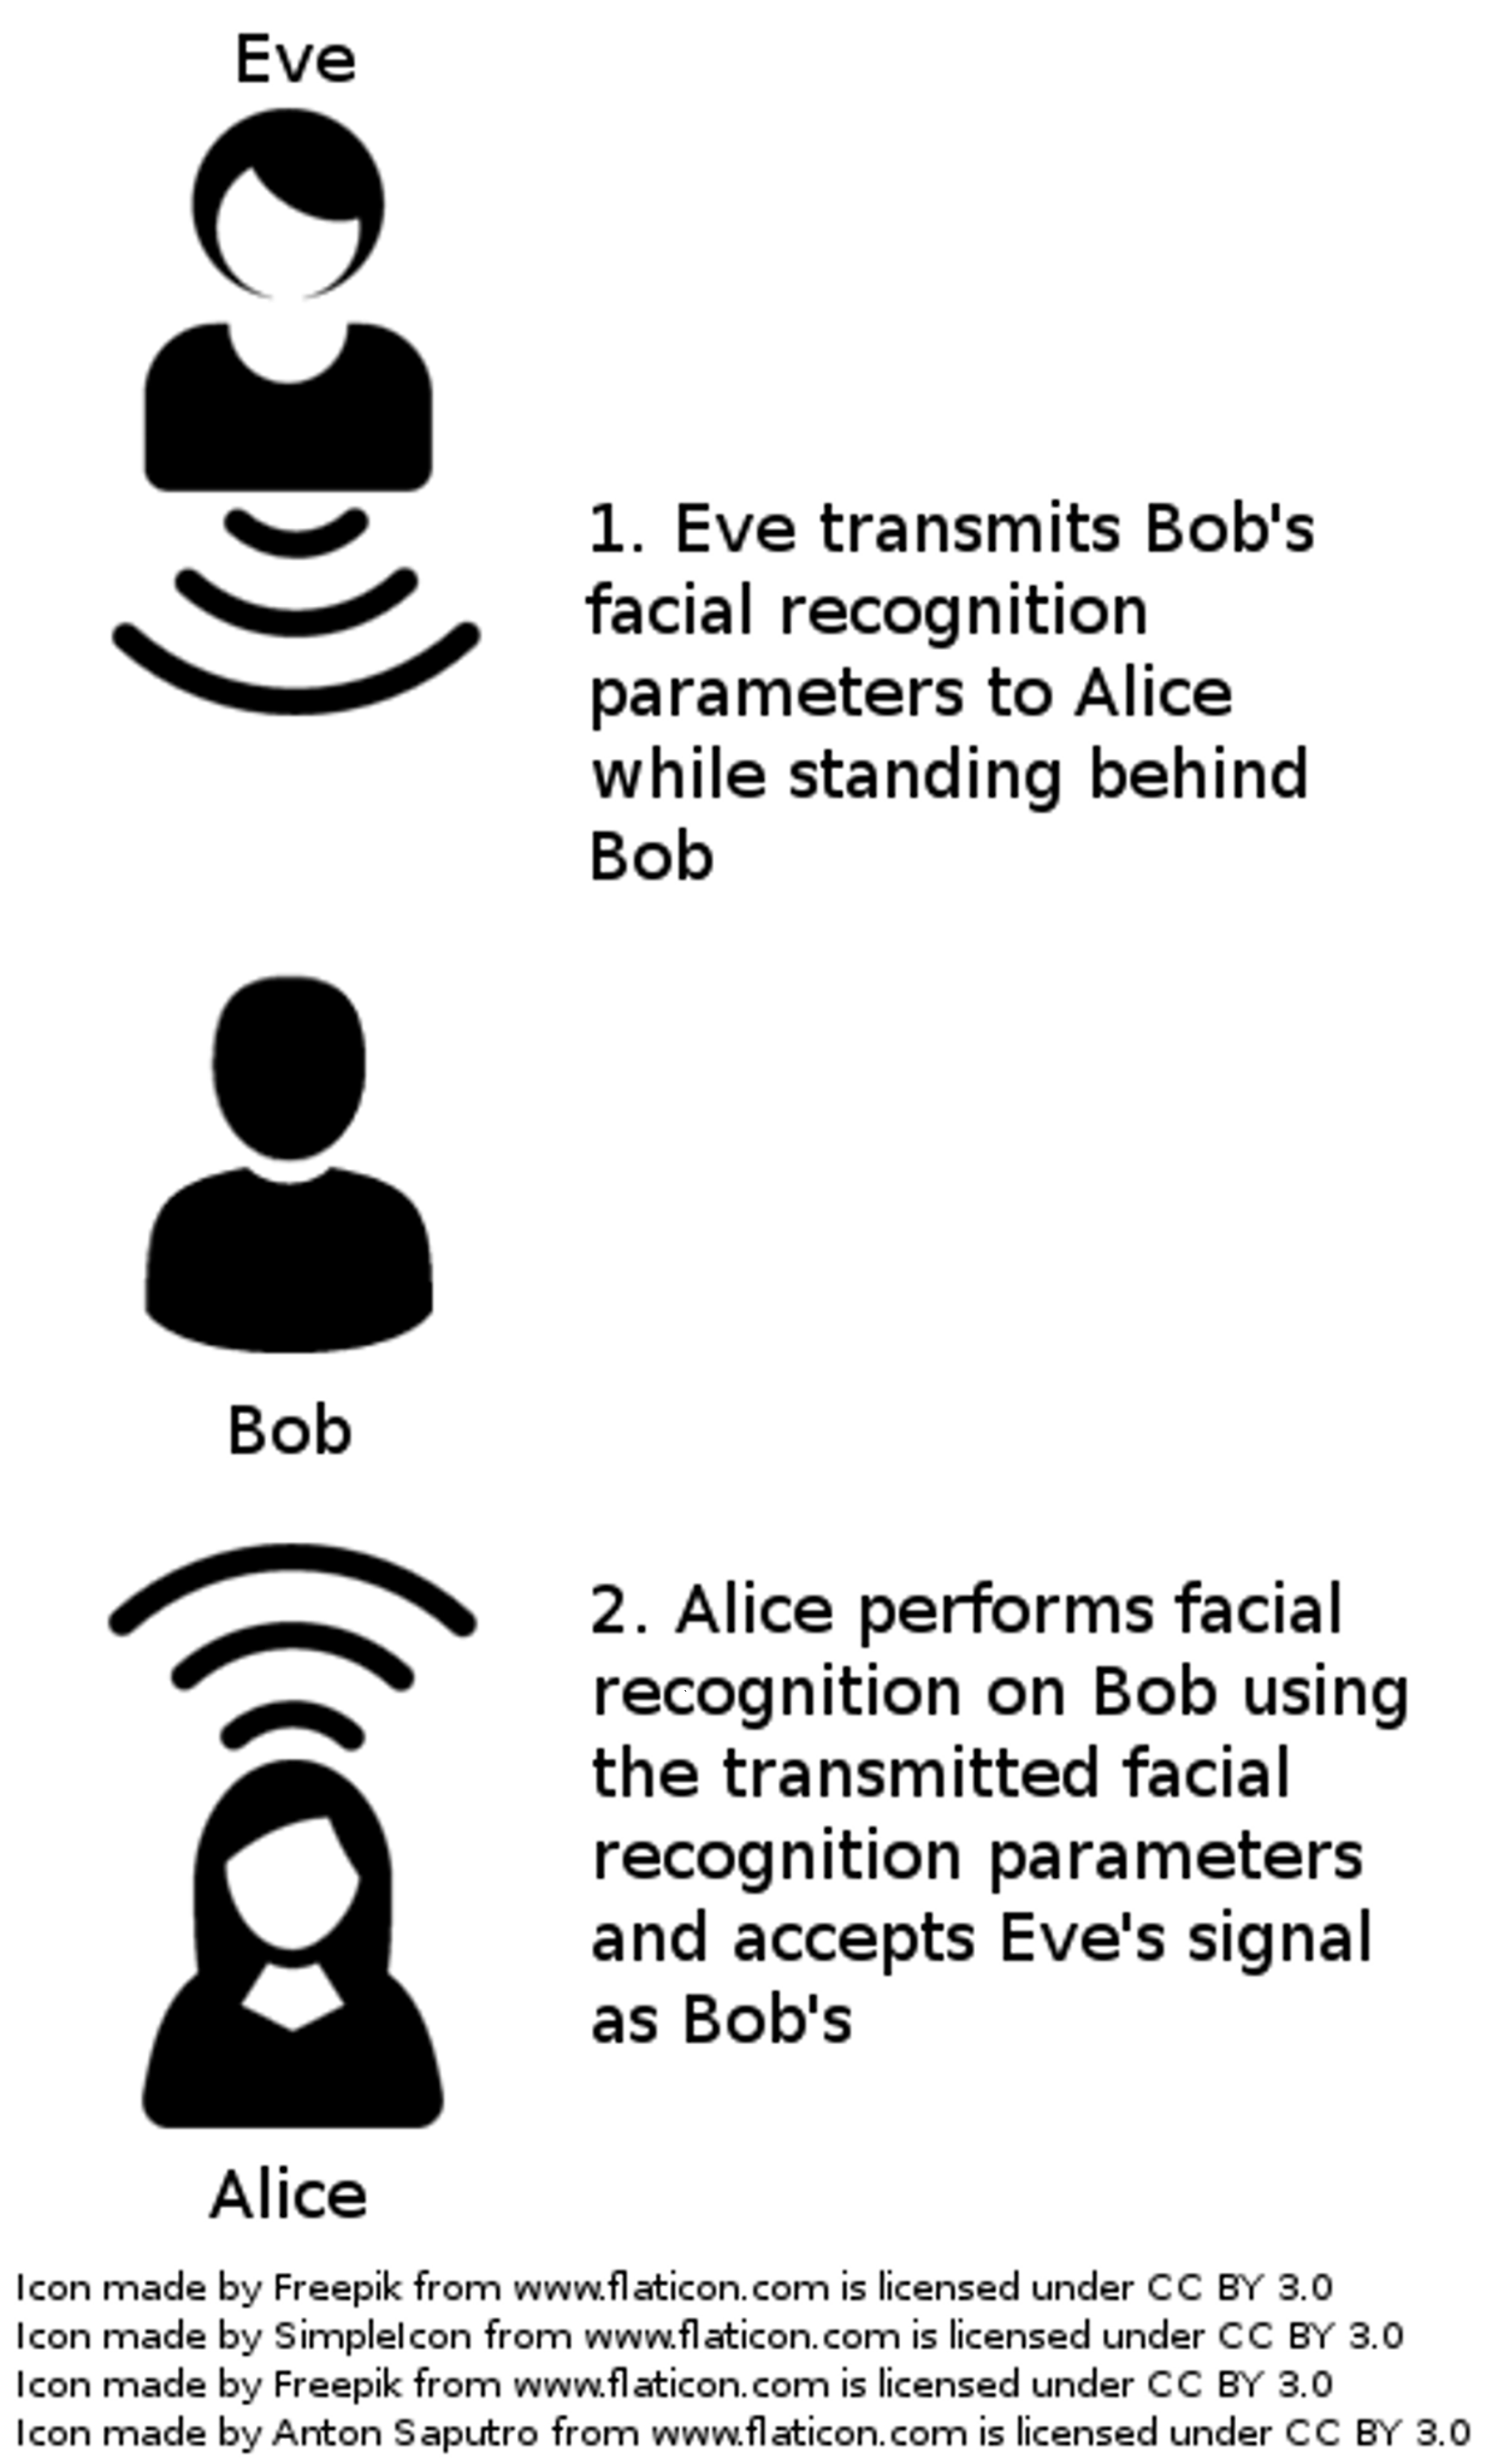
\includegraphics[scale=0.075]{../images/user-impersonation-attack.png}}
    \end{center}
\end{figure}

User impersonation will usually be protected against even further by context. LGTM's most likely use-case is that Alice and Bob want to share digital content via their augmented reality headsets and that they are already interacting and conversing. If Eve impersonates Alice to Bob, then Alice will not be sharing anything with Bob and vice-versa, which will not go unnoticed. Bob will likely terminate the connection and try again since it will be apparent that the protocol failed. This is slightly similar to pairing protocols which use an out-of-band channel to transmit authentication information, except in this case the out-of-band channel is being used for verification of a successful pairing. It is possible though to imagine scenarios where Bob might not notice that he is paired with someone besides Alice. Perhaps for some reason Alice and Bob are only pairing their devices and not communicating outside of that interaction. In this scenario, Eve's impersonation will succeed. It is our hope that wireless localization will continue to grow more and more precise, as it has over its entire history, to the point where inaccurate localization is no longer a valid attack vector. \par

Denial-of-service attacks are a common attack across pretty much all devices with network connectivity. Here we discuss two different ways that denial-of-service attacks can be launched against LGTM. The first is common to all wireless devices, jamming the wireless channel so that messages are not successfully received at all. There aren't any practical defenses against jamming, and thus it succeeds against LGTM. It is worth noting though that jamming requires expensive equipment and that it is illegal in many countries. \par

The second avenue for denial-of-service is through the protocol itself. LGTM has fairly expensive steps, particularly the localization step. If Eve spams Alice or Bob's device with LGTM requests, they will waste significant time processing these requests. But this attack goes further. Since these augmented reality headsets are stand-alone and mobile, they will be battery-powered. By spamming Alice or Bob's device and forcing heavy computation, Eve can execute a battery drain attack. The best defense against an attack like this is to have some sort of monitoring on LGTM protocol messages, and if too many are received, the protocol can be aborted. This is similar to TCP's congestion control mechanism \cite{TcpCongestionControl2009}. This prevents battery drain attacks, but does nothing to stop the denial-of-service attack. There is no way to really defend against this attack either. \par

When implemented properly, LGTM is very secure against the most common attacks on pairing protocols: man-in-the middle and user impersonation attacks. This security is, however, reliant on the accuracy of the implementation's wireless localization technique, but we expect the accuracy of wireless localization techniques to continue to increase. In fact, in the time between the start of work on this research and now a new technique was published \cite{ChronosSingleAPLocalizationVasisht2016}, bringing another leap forward in wireless localization. \par

% TODO: Comparison with Other Techniques (pin?)

\subsection{Usability}
Usability is a great thing to have for any piece of technology. It increases the likelihood of adoption, decreases avoidable user error, and reduces user frustration, which is linked to the other two points. \par

The International Standards Organization defines usability as, ``The extent to which a product can be used by specified users to achieve specified goals with effectiveness, efficiency, and satisfaction in a specified context of use'' \cite{UsabilityISO1998}. Besides being good for user satisfaction, usability can be an important factor in increasing security by reducing user errors that lead to security issues. It is no surprise that usability is increasingly becoming a focus for security schemes, especially in pairing \cite{UsabilitySecurityOutOfBandPairingKainda2009,UserPerceptionPairing,PlayfulPairingGallego2011,AliceMeetsBobKumar2009,SecurePairingUsabilityUzun2007,ConferenceCompStudySecurePairingKumar2009}. One study of device pairing methods \cite{SecurePairingUsabilityUzun2007} found that increasing the quality and usability of a user interface in a security scheme decreased errors that lead to a security failure in one pairing method by 20 percentage points and another by 7.5 percentage points. These two pairing methods were not seemingly complex schemes either. The first one required comparing two short alphanumeric strings on each device and confirming that they matched. The second one required selecting matching alphanumeric strings from a list on each device. It's also important to note that in this study, the devices were under the control of a single user. In \cite{AliceMeetsBobKumar2009} device pairing schemes with two users are examined. It was found that numeric-comparison had no fatal errors, but copy-confirm, where one user reads out a number to the other, and the other user then enters that number into their device, had a fatal error rate of 17\%. \par

To improve user satisfaction and increase security, LGTM is designed to be a highly usable security scheme that is both a pleasure to use and difficult to make security errors with. Combining facial recognition and wireless localization to reduce user-device authentication to two actions is very user-friendly. By adding facial recognition on top of wireless localization LGTM can auto-remove choices whose wireless signal location and face location do not match up. Users outside the device user's field of view are also auto-eliminated by context since the user is not facing that direction. Reducing the number of choices available to a user is a fantastic way to increase usability. When we consider the device pairing usability study mentioned above, we see that reducing the number of user choices should also reduce user error, since there are fewer wrong choices. Consider further that instead of recognizing a string of numbers, users are recognizing human faces, a particular human talent \cite{NewbornsFaceRecognitionTurati2006}. LGTM's combination of facial recognition and wireless localization makes for a very usable scheme that will also help prevent users from making security errors during authentication. \par

Usability is also impacted by the communications method used for LGTM. Point to point device communication is always available, barring local device failures, which inherently makes it more usable since it can be used in a larger variety of scenarios. Consider the common case of being on an airplane with no reliable wireless connection or the even more common case of being in an area with no WiFi and no cellular connection. This second case is present every day for many people in both rural and undeveloped areas with slow or nonexistent Internet connections, and as a result, sharing content with people who are present by going over the Internet would range from prohibitively time consuming to impossible. \par
% Usability is good for users (for products, etc)
% Usability impacts security
% ---- Examples: Phishing, case studies, trojans, click-bait, etc

% Facial recognition improves usability
% ---- Bring up alternative localization sphere
% ---- Humans have a fantastic ability to recognize faces (bringing up AGAIN)
% ---- In standard case (non-malicious) selections can be auto-eliminated if faces & localization don't line up, leading to fewer user choices, which is always more usable
% -------- Link back to usability leading to more security

% Wireless p2p improves usability
% ---- ALWAYS available
% -------- No Internet, no problem
% -------- Bring up relatable analogies (on the plane, basic lack of service, geographically lacking quality service (rural areas, Kansas))
% ---- Centralized infrastructure requires secondary authentication
% -------- "Yo dawg, you need to authenticate so you can authenticate"
% -------- This is LESS usable, more steps, more room for mistakes, more room for bugs (security tie in again?)

% LGTM Approaches MAX usability
% ---- It's how we authenticate human speakers!
% ---- Only two user actions, begin, and confirm (how can you reduce from that?)


\subsection{Privacy} % (This will not be a particularly long sub-section...)
A common misconception is that most people are not concerned about digital privacy. However, a 2015 study by the Pew Research Center \cite{AmericanPrivacyOnlinePew2015} found that 86\% of Internet users have taken steps to remove or mask their digital footprints online, and 55\% of Internet users have taken steps to avoid surveillance by specific individuals, organizations, or governments. When it comes to user privacy, LGTM delivers. Since LGTM relies on point to point wireless communication, attackers must be co-located with their targets, significantly diminishing the reach that arbitrary attackers can exert. Prolonged digital surveillance of an individual's point to point content sharing would require something akin to stalking, which we believe is unlikely to occur as often as hacking does on the Internet. \par

Furthermore, by sending data from point to point, we avoid empowering a central authority with hordes of user data: who users talk to, who users are close to, what users are sending to one another, and when. This is data that many users would like to keep private, but that many large companies see as a gold mine. The safest way to keep this data from being abused is not to make it available to third-parties. With LGTM, this data is as private as any untapped conversation between two people. \par


\chapter{Implementation}
\section{Testbed}
Real world augmented reality headsets are still fresh on the market and are very rare. On top of this, the few headsets on the market do not provide sufficient access to information about the wireless channel that is necessary for wireless localization. These two factors make implementing LGTM on real augmented reality headsets infeasible. \par

However, we have stripped down LGTM's hardware requirements to the bare minimum leaving us in need of: a high-definition video camera, wireless point to point communication capabilities, wireless localization capabilities, a display, reasonable computational abilities, and close proximity of a face to wireless antennas. We satisfy all of these requirements by equipping two Fujitsu LifeBook T900 laptops running Linux Mint 17 Qiana with a Logitech C270 720p web cam, an Intel 5300 wireless card with custom firmware for Linux from Halperin et al. \cite{ChannelStateInformationToolReleaseHalperin2011} that enables retrieval of channel state information and point to point wireless communication using 802.11n, an array of three antennas affixed to the back of the laptop screen at 10 centimeter intervals, and finally by attaching printed pictures of faces from the Yalefaces dataset \cite{FisherfacesBelhumeur1997} to the back of the laptop over the antenna array. This last point is important since augmented reality headset users will have their face directly adjacent to the wireless transmitter which LGTM exploits to couple the wireless signal and the user together. This context is an extremely important enabler of LGTM. To be sure, our testbed itself is not a practical setup, but it perfectly emulates the requisite hardware of real augmented reality headsets. \par

\begin{figure}[!htb]
    \begin{center}
        \caption{Testbed laptop shown without a printed picture of a face and with a printed picture of a face.}
        \label{figure: testbed-pictures}
        \begin{subfigure}[Testbed without face picture attached]{0.3\textwidth}
            \centerline{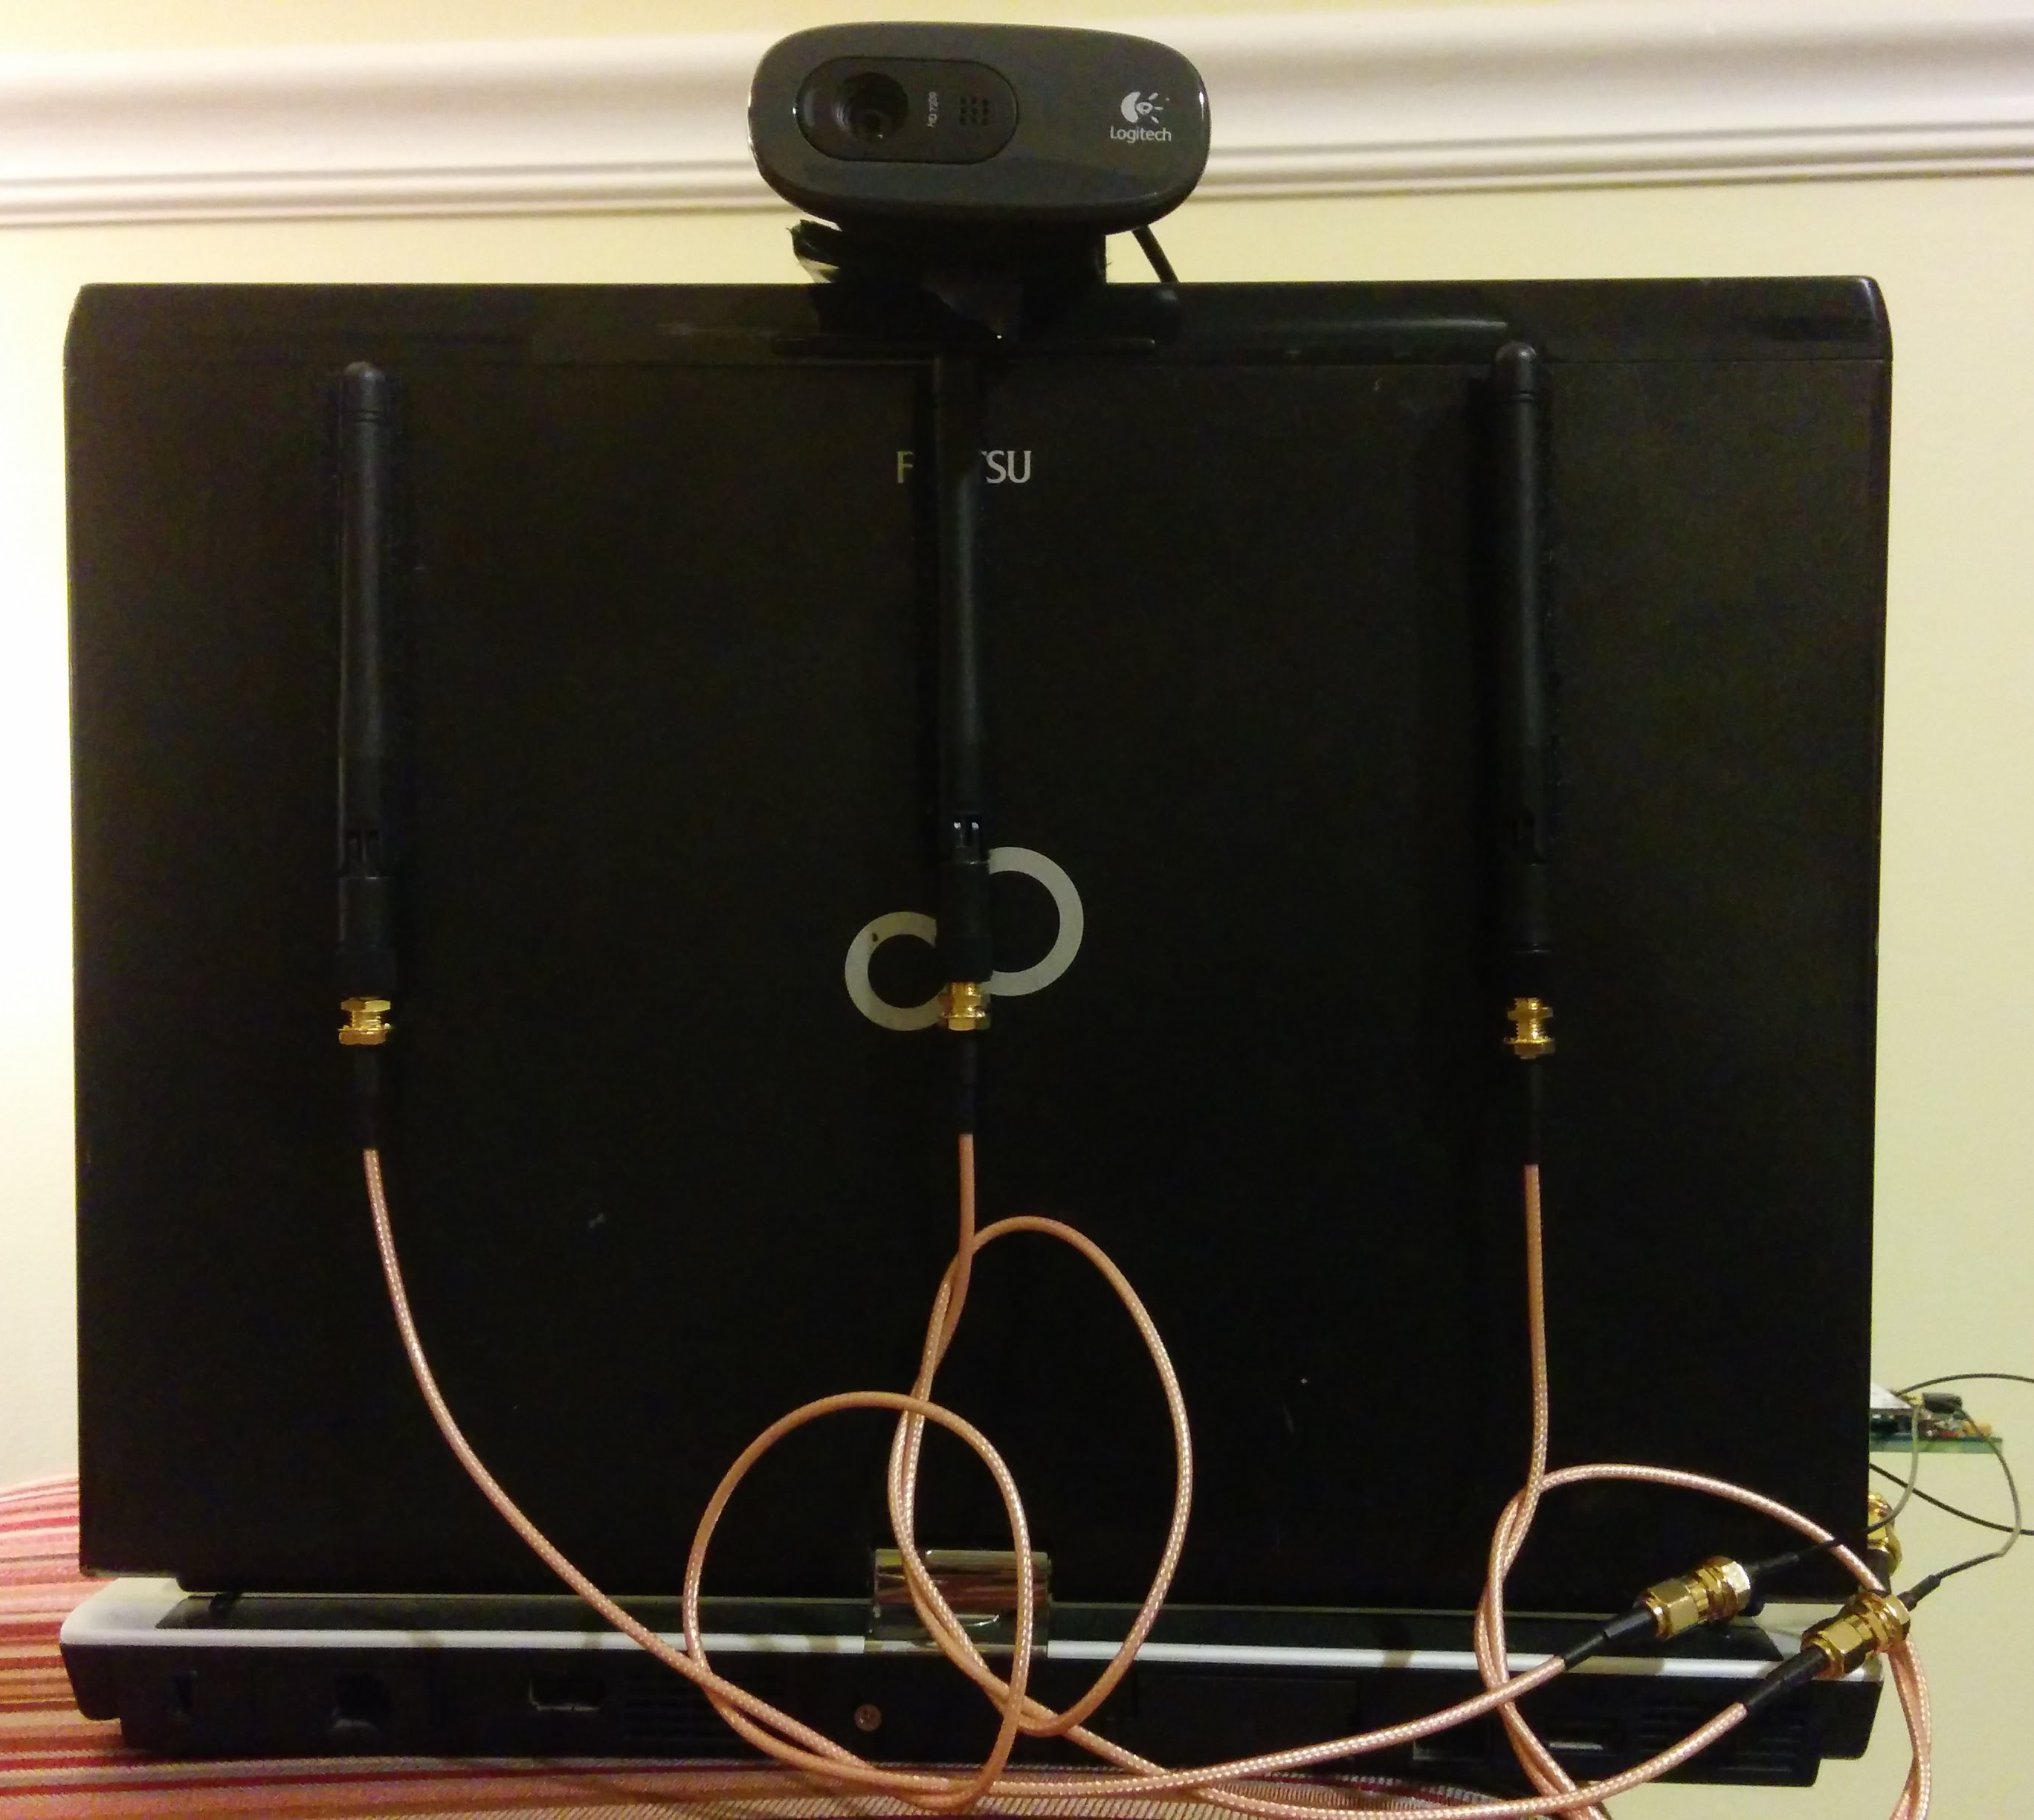
\includegraphics[scale=0.1]{../images/testbed-without-face.jpg}}
        \end{subfigure}
        \par\bigskip
        \begin{subfigure}[Testbed with face picture attached]{0.3\textwidth}
            \centerline{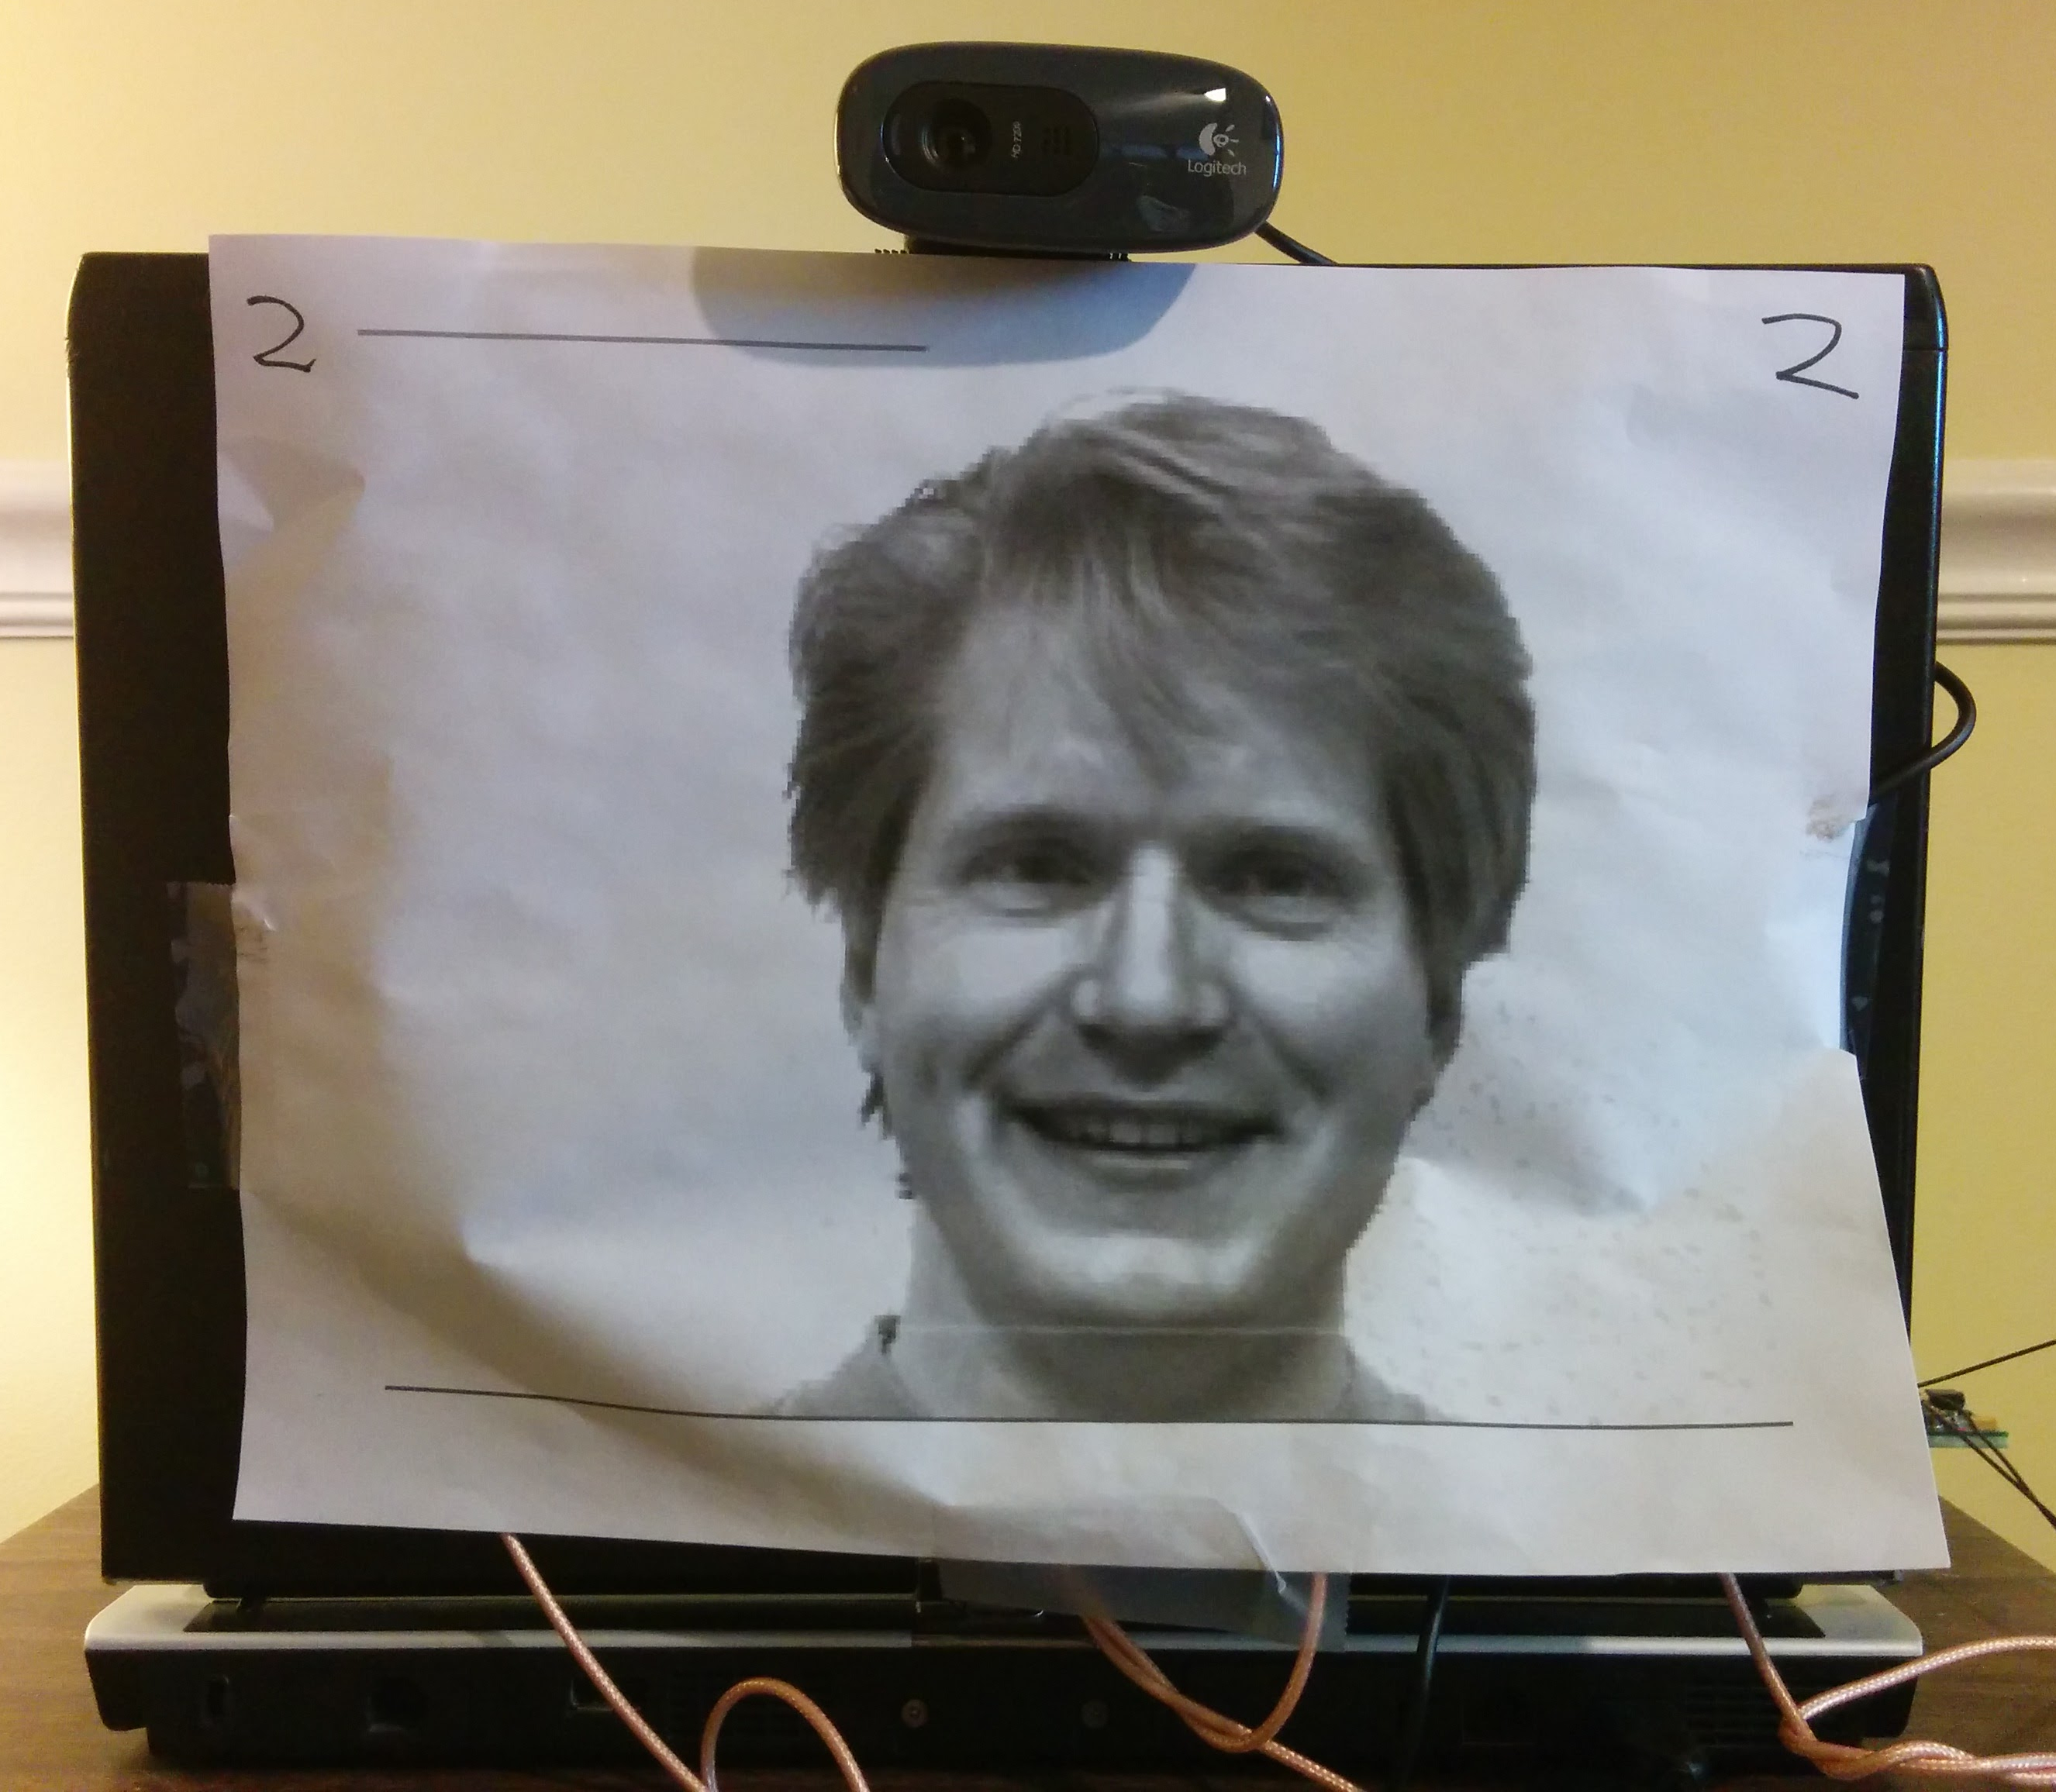
\includegraphics[scale=0.1]{../images/testbed-with-face.jpg}}
        \end{subfigure}
        \par\bigskip
    \end{center}
\end{figure}
% Why LGTM cannot be implemented on real AR systems
% ---- Availability
% ---- Lack of open firmware for wireless localization
% My solution
% ---- Necessary conditions for LGTM that AR satisfies:
% -------- High-definition video camera
% -------- Wireless p2p communications capabilities
% -------- Wireless localization capabilities
% -------- Proximity of face to wireless communications
% -------- Screen
% -------- Computational abilities
% ---- Web cam
% ---- Wireless card with open firmware to grab CSI
% ---- array of 3 antennas
% ---- Pictures of faces on top of the arrays
% ---- Laptop

% Hardware section from My Thesis is included and shortened and put under testbed here
% Laptops + specs + OS
% Wireless cards
% ---- Explain why the Intel 5300 was chosen
% -------- Firmware
% -------- Extra software
% -------- More elaboration under software section
% Antennas
% ---- Spacing
% ---- Positioning on laptops 
% ---- Location relative to face print outs
% Web cams
% ---- Manufacturer information + model
% ---- Field of view
% ---- Resolution
% ---- Frame rate

\section{Technologies and Software}
% Encryption
% ---- Elliptic-Curve Ephemeral Diffie-Hellman
% ---- SHA-512 (for message stream authentication (like a secure session id))
% ---- AES-128 GCM (authentication + encryption)

% Facial Detection & Recognition
% ---- Haarcascades
% ---- LBPH
LGTM employs many technologies in service of bootstrapping secure communication, and these technologies have several different implementation choices. \par

\subsection{Wireless Communication}
We use the 5 GHz channel of 802.11n as our wireless channel. There are known issues that arise with the Intel 5300 wireless card and the channel state information the custom firmware provides when it is operated on the 2.4 GHz channel \cite{PhaserGjengset2014,SpotFiKotaru2015}. To listen to the channel and send and receive packets, we use the existing supplementary software for the Intel 5300 CSI Tool \cite{ChannelStateInformationToolReleaseHalperin2011}. We make some minor modifications to the existing code to handle packet decoding in addition to channel state information recording and to facilitate reading data from files to be transmitted. The supplementary software is written in a combination of MATLAB and C. To configure the wireless card and OS settings, we use the Linux networking `ip' command and wireless networking `iw' command extensively. \par

\subsection{Cryptography}
\subsubsection{Technologies}
In our implementation, we employ elliptic curve Diffie-Hellman key exchange instead of standard Diffie-Hellman key exchange to reduce the number of bits required for the public-private key pairs, thus increasing performance \cite{FastEllipticCurveDiffieHellmanBernstein2006}. Elliptic curve Diffie-Hellman requires an appropriate elliptical curve to perform computations over, and we use curve secp256r1, specified in \cite{EllipticCurvesStandard2009}. This curve is used by default in our implementation, so there is no agreement step to come to a consensus between the devices involved, and the parameters $g$ and $p$ in \ref{figure: protocol-diagram} are not transmitted. \par

For symmetric encryption, we use the advanced encryption standard (AES) block cipher with a 128 bit key \cite{AesNist2001} in Galois Counter Mode (GCM) \cite{GcmModeMcGrewNist2005}. Galois counter mode provides both authentication and encryption for messages by using a keyed hash as a message authentication code or HMAC for short. GCM operates only over block ciphers with 128-bit blocks, hence our choice of AES-128 over AES-256. \par

\subsubsection{Software}
To implement LGTM's cryptographic components we use the popular Crypto++ C++ library, which provides functions and classes to support elliptic-curve Diffie-Hellman, random number generation, AES, and Galois counter mode for various symmetric key algorithms. \par

Using these crypto-primitives, I built up two main files: one to run the cryptographic building blocks of LGTM and one to use these building blocks to form the messages sent back and forth between Alice and Bob. The cryptographic building blocks for LGTM are separated into 6 functions: 

\begin{itemize}
    \item generateRandomNumber
    \item generateDiffieHellmanParameters
    \item diffieHellmanSharedSecretAgreement, 
    \item generateSymmetricKeyFromSharedSecret
    \item encryptFile
    \item decryptFile
\end{itemize}

The function names should be mostly self-explanatory; they serve to generate a random number and return it, generate a public-private key pair for Diffie-Hellman and return them, agree on a shared key using Diffie-Hellman, generate a symmetric key using the shared secret, and encrypt and decrypt files. In my implementation, these functions can be found under the cryptography folder in the lgtm\_crypto.cpp file. \par

These functions are used by the higher level functions that construct messages to send at each step of the protocol. These messages can all be mapped back to steps in the protocol diagram in figure \ref{figure: protocol-diagram}. Their names are: 

\begin{itemize}
    \item firstMessage
    \item replyToFirstMessage
    \item secondMessage
    \item replyToSecondMessage
    \item decryptThirdMessageReply
\end{itemize}

FirstMessage generates a Diffie-Hellman public-private key pair, generates a random number that's 256 bits long, and writes the random number and public key to a single file as well as writing all the generated data to separate files for retrieval later. ReplyToFirstMessage splits a received file into the random number and public key from firstMessage, generates a public-private key pair, derives the shared secret and symmetric key using the other public key, generates a random number, exclusive-ors the generated random number and the received random number together, then writes the generated parameters to separate files and the generated public key, random number, and exclusive-or of both random numbers to a single file. \par

SecondMessage splits a received file into the random number, public key, and exclusive-or of both random numbers. Then it derives the Diffie-Hellman shared secret, computes a symmetric key using the Diffie-Hellman secret, writes all the newly generated parameters to separate files, and encrypts and saves a file using the shared symmetric key that holds data to be used for facial recognition. \par

ReplyToSecondMessage decrypts and saves a received message, exiting with a failure status if the encrypted data is found to have been tampered with. Then it encrypts a file using the shared symmetric key holding data to be used for facial recognition and saves it. \par

Finally, decryptSecondMessageReply decrypts and saves a received file, exiting with a failure status if the encrypted data is found to have been tampered with. \par

These various methods are are invoked from the command line by passing the following string arguments to the program: 

\begin{itemize}
    \item first-message
    \item first-message-reply
    \item second-message
    \item second-message-reply
    \item decrypt-third-message-reply
\end{itemize}

In my implementation, these functions can be found under the cryptography folder in the lgtm\_crypto\_runner.cpp file. \par

Data is passed and stored primarily using files. The reasoning behind this is that the cryptography software for LGTM is run periodically as part of the higher-level LGTM program. As a result, we must maintain state variables between runs where the program exits as well as reading in data generated by other separate programs. The simplest way to do this is through files. \par

\subsection{Facial Recognition}
Facial recognition is a multi-step process. Before recognizing a face, all the faces in the current field-of-view must be detected. Our implementation detects all faces in the current field of view and then checks each one with facial recognition. Our implementation's facial detection relies upon Haar feature-based cascade classifiers \cite{HaarCascadeViola2001}. This method was designed specifically for performance. It uses many feature detectors that are run in a tree-like fashion, with simpler, faster feature detectors being run first, followed by more complex, more expensive, more discriminating feature detectors. \par

To recognize the faces detected, we require robust facial recognition under sometimes less than ideal circumstances. Most facial recognition algorithms are tested using image files directly fed into the algorithm. Oftentimes these images are taken under idealized conditions that are not necessarily representative of common use-cases. As a result, we found that several facial recognition algorithms are not sufficiently robust to serve our purposes. In our testbed, we are running facial recognition on images from the Yalefaces dataset attached to laptops, but our training set of images is comprised of image files from the Yalefaces \cite{FisherfacesBelhumeur1997} dataset. So we need a facial recognition algorithm that can generalize from faces in photos taken in idealized conditions to the less than ideal case we face in our testbed of recognizing faces in photos affixed to laptops. To serve this need, we use linear binary pattern histograms (LBPH) for facial recognition \cite{LBPHAhonen2004,LearningMultiScalBlockLBPHLiao2007}. This technique has been found to be robust in many conditions where facial recognition techniques based on more elegant methods, such as Eigenfaces \cite{EigenfacesTurk1991} and Fisherfaces \cite{FisherfacesBelhumeur1997}, fail. Our cursory evaluation of facial recognition techniques indeed found that Eigenfaces and Fisherfaces were insufficient for our applications, recognizing approximately half of the faces in Yalefaces, while LBPH succeeds in recognizing all the faces in Yalefaces. \par

We used the OpenCV 3.0 \cite{OpenCV} C++ library in our implementation to compare Eigenfaces, Fisherfaces, and LBPH for facial recognition and also for facial detection using Haar feature-based cascade classifiers. OpenCV provides out-of-the-box implementations for all of these methods. \par

I put together these components, and others, to implement LGTM. The Yalefaces dataset is preprocessed before the training sets for each individual is put together. This preprocessing step crops the image to include the face and as little else as possible. This was done using the Haar cascade classifier on each image and then cropping on the detected face. I experimented with data augmentation techniques to increase the size of the dataset. Specifically, I perturbed each training image by many combinations of angles along all three axes. Unfortunately this did not create a better classifier for my use-case, in fact, it made it worse. This was true for Eigenfaces, Fisherfaces, and LBPH. \par

When LGTM is being run, I retrain an LBPH classifier using a newly received set of photos of one of the individuals from the Yalefaces dataset. This retraining takes less than 1 second, so it is not a significant contributor to the computational cost of running LGTM. \par

\subsection{Wireless Localization}
The most intricate of the technologies involved in LGTM is by far wireless localization. The recent advances in wireless localization \cite{UbicarseKumar2014,SpotFiKotaru2015,ChronosSingleAPLocalizationVasisht2016} are indeed what make LGTM feasible. For our testbed, we implemented a modified version of SpotFi \cite{SpotFiKotaru2015}, adapted to run from a single device instead of coordinated devices. SpotFi is an angle of arrival based localization technique that relies on the classical MUSIC algorithm \cite{MUSICSchmidt1986} to compute the angle that a wireless signal originates from relative to an array of antennas. 

\subsubsection{MUSIC}
The key to MUSIC is the existence of a phase difference between each signal as it arrives at each antenna in an array. These phase differences occur because the antennas are at different locations, meaning a single wireless signal must travel different distances to arrive at each antenna in an antenna array, thus causing a phase difference. When expressed as a complex exponential we can write the signal at the Nth antenna as:

$$\Phi(\theta_{k}) = e^{-j 2 \pi d \frac{sin(\theta_{k}) f}{c}}$$

where $j$ is $\sqrt{-1}$, $f$ is the wireless signal's frequency, $d$ is the distance between antennas in the array, $c$ is the speed of light, and $\theta_k$ is the angle of arrival for path $k$. The vector of these expressions is referred to as the steering vector, denoted $a(\theta)$, and is a function of $\theta$ since the remaining parameters are constant. \par

\begin{figure}
    \begin{center}
        \caption{The steering vector form used in music. Each element indicates the phase offset from the first antenna in an array, which is why the first element is 1. Since the antennas in the array are spaced at a constant distance, $d$, the phase offset at each array element is a multiplicative increase.}
        \label{figure: music-steering-vector}
        $\begin{bmatrix}
        1 \\
        e^{-j 2 \pi d \frac{sin(\theta_{k}) f}{c}} \\
        e^{2 * (-j 2 \pi d \frac{sin(\theta_{k}) f}{c})} \\
        ... \\
        e^{(M - 1) * (-j 2 \pi d \frac{sin(\theta_{k}) f}{c})} \\
        \end{bmatrix}$
    \end{center}
\end{figure}

The MUSIC paper models a received wireless signal, the column vector $X$ with $M$ elements, in terms of a matrix, $A$, with $D$ columns, each of which is a steering vector parameterized with a different $\theta$. The $D$ steering vectors are for the $D$ different signal paths resulting from multipath effects. Each of these steering vectors has $M$ elements, one for each antenna, making $A$ an $M \times D$ matrix. This matrix is multiplied by a column vector of $D$ complex gains, and this expressions has Gaussian white noise added to it. All this is written as:

$$X = AF + W$$

For the purpose of localization, we seek to compute $A$ from the information we have about the physical layer through our setup and the measured signal, $X$. To start with, MUSIC computes the covariance matrix $S = XX^{H} = A FF^{H} A^{*} + WW^{H}$, where $H$ denotes the conjugate transpose. This expression is decomposed using eigendecomposition so that we get: $S = A FF^{H} A^{H} + \lambda S_{0}$, where $S_{0}$ represents noise and $\lambda$ is an eigenvalue of $S$. When the elements of the noise vector $W$ have mean 0 and variance $\sigma^{2}$ $\lambda S_{0} = \sigma^{2} I$, where $I$ is the identity matrix. When the number of paths, $D$, is less than the number of sensors, or in our case antennas, $M$, then $A FF^{H} A^{H}$ is singular, making its determinant 0. This insight yields the expression:

$$\lvert A FF^{H} A^{H} \rvert = \lvert S - \lambda S_{0} \rvert = 0$$

If $A$ is a full rank matrix and $FF^{H}$ is positive definite then $A FF^{H} A^{H}$ must be a positive semi-definite matrix, meaning that the $\lambda$ in the expression above must be the minimum eigenvalue $\lambda_{min} \geq 0$. \par

The rank of $A FF^{H} A^{H}$ is $D$ and this can be shown by computing the eigenvalues of $S$, since $\lambda_{min}$ will be repeated $P = M - D$ times. Using this we can compute the number of paths, $D$, from measurements by determining $P$ by counting the number of times the minimum eigenvalue is repeated for $S$. \par

Back to our steering vectors. Recall that there are $D$ actual angle of arrivals from multipath. When these true angle of arrivals are input to the steering vector, it will be orthogonal to what is referred to as the noise sub-space. MUSIC computes the noise sub-space by computing the eigenvectors of the signal covariance matrix and constructing a new matrix using the eigenvectors whose eigenvalues are at a minimum as columns. There are $P$ such eigenvectors. This matrix is denoted $E_{N}$. \par

To use MUSIC for computing the angle of arrival, we compute $P_{MUSIC}(\theta) = \frac{1}{a^{*}(\theta) E_{N} E_{N}^{*} a(\theta)}$ for a range of $\theta$ values and see where $P_{MUSIC}$ peaks. The largest peak is the direct path angle of arrival. \par

\subsubsection{SpotFi}
Due to multipath effects, there will usually be multiple peaks. Multipath is resolved in MUSIC by having more sensors, which in our case are antennas. Specifically, the number of sensors in MUSIC must be more than the number of multipath components. However, average indoor conditions usually have five paths resulting from multipath effects, and having five or more antennas on a consumer device is currently impractical and expensive. \par

The key insights in SpotFi to overcome limitations from multipath and a limited number of antennas are using channel state information measurements from each subcarrier in 802.11n combined with a method of creating more sensors using mathematical tricks while requiring only three antennas. \par

To understand this first insight, let's briefly look at what subcarriers and how they're used. Many modern communications systems, including 802.11n, rely on a scheme called orthogonal frequency division multiplexing (OFDM). From a high level, OFDM divides up a band of frequency into separate channels and transmits different data using each channel. These separated channels are referred to as subcarriers since each has a carrier frequency which is a small part of a different central frequency which defines the section used for OFDM. OFDM selects subcarriers whose frequencies are closely spaced, but also orthogonal to minimize interference. The primary advantage of OFDM is its ability to cope with poor channel conditions. $<GET \: A \: GOOD \: FIGURE \: FOR \: THIS>$ $[CITATION \: TOO]$. \par

To use these subcarriers first requires a modification to the model of a wireless signal presented in the original MUSIC paper. Instead of modeling $X$ as a column vector of $M$ measurements, from $M$ antennas, we model $X$ as an $M \times N$ matrix, where $N$ equals the number of subcarriers used. This results in the channel gain matrix $F$ being modeled as a $D \times N$ matrix and the noise matrix $W$ being modeled as a $M \times N$ matrix. \par

The authors of SpotFi perform their manipulations on the expression, minus the noise matrix, $W$, for simplicity, so I will do the same for the remainder of this explanation of SpotFi. \par

SpotFi modifies MUSIC to use steering vectors that consider both time of flight and angle of arrival. As stated above, MUSIC uses phase differences across sensor arrays; phase differences between subcarriers are too small to be useful since the difference is $2 \pi (m - 1) d (f_i - f_j) \sin(\theta_k) / c$, where $f_i$ and $f_j$ denote the frequencies of two subcarriers. This phase difference is rendered insignificant by the speed of light term, $c$, in the denominator. The maximum spacing between subcarriers in 802.11 is 40 MHz. At this distance, with antennas spaced at half a wavelength, any angle of arrival introduces a phase shift of at most 0.002 radians across the subcarriers, which can easily be a result of noise. The authors of SpotFi introduce time of flight to obtain more discriminating phase differences. Time of flight between subcarriers can also be expressed as a complex exponential:

$$\Omega(\tau_{k}) = e^{-j 2 \pi f_{\delta} \tau_k }$$

where $f_{\delta}$ is the frequency difference between subcarriers and $\tau_{k}$ is the time of flight for the kth path. The phase difference for time of flight across two adjacent subcarriers can be computed with: $-2 \pi (n - 1) f_{\delta} \tau_k$, where $f_{\delta}$ is the frequency difference between two adjacent subcarriers. Since there is no speed of light term in the denominator,  the phase difference that exists between subcarriers is significant. SpotFi uses these phase differences between subcarriers for time of flight the same way classical MUSIC uses the phase differences between antennas. \par

However, to properly utilize the new time of flight phase shifts, some additional work must be done. Recall that MUSIC requires that the number of measurements from the sensor array that can be written as a linear combination of steering vectors must be greater than the number of paths. To satisfy this requirement, the SpotFi authors construct a new signal measurement matrix $X$ using the recorded signal information. \par

Recall that in the classical MUSIC algorithm, the steering vector is a vector of signals obtained across an antenna array that is parameterized only by an angle $\theta$. SpotFi's modification in adding time of flight makes the steering vector a two parameter function, $a(\theta, \tau)$, where $\tau$ is time of flight. However, the new steering vector and signal measurement matrix must be carefully manipulated to fit the constraints put forward by MUSIC. The trick to doing this is to construct the new $X$ such that the sensors are overlapping sub-arrays of sensors in terms of time of flight and angle of arrival. 

% TODO: More detail

Since MUSIC is a mathematical technique, the authors of SpotFi move $\Phi_{\theta k}$ and $\Omega_{\tau k}$ terms into the matrix of complex gains, $F$, so that $A$ can be expressed in terms of steering vectors whose only difference is the values of $\theta$ and $\tau$ that they're parameterized by. 

% TODO: More detail

\begin{figure}[!htb]
    \begin{center}
        \caption{}
        \label{figure: spotfi-smoothing-explained}
        \begin{subfigure}[b]{0.3\textwidth}
            \caption{}
            \label{subfigure: smoothed-csi-matrix}
            \centerline{\scalebox{0.5}{$
X
=
\begin{bmatrix}
csi_{1,1} & csi_{1,2} & ... & csi_{1, 16} & csi_{2, 1} & csi_{2, 2} & ... & csi_{2, 16} \\ 
csi_{1,2} & csi_{1,3} & ... & csi_{1, 17} & csi_{2, 2} & csi_{2, 3} & ... & csi_{2, 17} \\ 
. & . & . & . & . & . & . & . \\
. & . & . & . & . & . & . & . \\
. & . & . & . & . & . & . & . \\
csi_{1,15} & csi_{1,16} & ... & csi_{1, 30} & csi_{2, 15} & csi_{2, 16} & ... & csi_{2, 30} \\ 
csi_{2,1} & csi_{2,2} & ... & csi_{2, 16} & csi_{3, 1} & csi_{3, 2} & ... & csi_{3, 16} \\
csi_{2,2} & csi_{2,3} & ... & csi_{2, 17} & csi_{3, 2} & csi_{3, 3} & ... & csi_{3, 17} \\  
. & . & . & . & . & . & . & . \\
. & . & . & . & . & . & . & . \\
. & . & . & . & . & . & . & . \\
csi_{2,15} & csi_{2,16} & ... & csi_{2, 30} & csi_{3, 15} & csi_{3, 16} & ... & csi_{3, 30} \\ 
\end{bmatrix}$}}
        \end{subfigure}
        \par\bigskip
        \begin{subfigure}[b]{0.3\textwidth}
            \caption{}
            \label{subfigure: steering-matrix}
            \centerline{\scalebox{0.5}{$
A
=
\begin{bmatrix}
1 & 1 & ... & 1 & 1 & 1 & ... & 1 \\
\Omega_{\tau 1} & \Omega_{\tau 2} & ... & \Omega_{\tau \frac{L}{2}} & \Omega_{\tau (\frac{L}{2} + 1)} & \Omega_{\tau (\frac{L}{2} + 2)} & ... & \Omega_{\tau L} \\
\Omega^{2}_{\tau 1} & \Omega^{2}_{\tau 2} & ... & \Omega^{2}_{\tau \frac{L}{2}} & \Omega^{2}_{\tau (\frac{L}{2} + 1)} & \Omega^{2}_{\tau (\frac{L}{2} + 2)} & ... & \Omega^{2}_{\tau L} \\
. & . & . & . & . & . & . & . \\
. & . & . & . & . & . & . & . \\
. & . & . & . & . & . & . & . \\
\Omega^{14}_{\tau 1} & \Omega^{14}_{\tau 2} & ... & \Omega^{14}_{\tau \frac{L}{2}} & \Omega^{14}_{\tau (\frac{L}{2} + 1)} & \Omega^{14}_{\tau (\frac{L}{2} + 2)} & ... & \Omega^{14}_{\tau L} \\
\Phi_{\theta 1} & \Phi_{\theta 2} & ... & \Phi_{\theta \frac{L}{2}} & \Phi_{\theta (\frac{L}{2} + 1)} & \Phi_{\theta (\frac{L}{2} + 2)} & ... & \Phi_{\theta L} \\
\Omega_{\tau 1} \Phi_{\theta 1} & \Omega_{\tau 2} \Phi_{\theta 2} & ... & \Omega_{\tau \frac{L}{2}} \Phi_{\theta \frac{L}{2}} & \Omega_{\tau (\frac{L}{2} + 1)} \Phi_{\theta (\frac{L}{2} + 1)} & \Omega_{\tau (\frac{L}{2} + 2)} \Phi_{\theta (\frac{L}{2} + 2)} & ... & \Omega_{\tau L} \Phi_{\theta L} \\
. & . & . & . & . & . & . & . \\
. & . & . & . & . & . & . & . \\
. & . & . & . & . & . & . & . \\
\Omega^{14}_{\tau 1} \Phi_{\theta 1} & \Omega^{14}_{\tau 2} \Phi_{\theta 2} & ... & \Omega^{14}_{\tau \frac{L}{2}} \Phi_{\theta \frac{L}{2}} & \Omega^{14}_{\tau (\frac{L}{2} + 1)} \Phi_{\theta (\frac{L}{2} + 1)} & \Omega^{14}_{\tau (\frac{L}{2} + 2)} \Phi_{\theta (\frac{L}{2} + 2)} & ... & \Omega^{14}_{\tau L} \Phi_{\theta L} \\
\end{bmatrix}$}}
        \end{subfigure}
        \par\bigskip
        \begin{subfigure}[b]{0.3\textwidth}
            \caption{}
            \label{subfigure: complex-gains-matrix}
            \centerline{\scalebox{0.5}{$
F
=
\begin{bmatrix}
\alpha_{1} & \alpha_{1} \Omega_{\tau_{1}} & \alpha_{1} \Omega^{2}_{\tau_{1}} & ... & \alpha_{1} \Omega^{15}_{\tau_{1}} & \alpha_{1} \Phi_{\theta_{1}} & \alpha_{1} \Omega_{\tau_{1}} \Phi_{\theta_{1}} & \alpha_{1} \Omega^{2}_{\tau_{1}} \Phi_{\theta_{1}} & ... & \alpha_{1} \Omega^{15}_{\tau_{1}} \Phi_{\theta_{1}} \\
\alpha_{2} & \alpha_{2} \Omega_{\tau_{2}} & \alpha_{2} \Omega^{2}_{\tau_{2}} & ... & \alpha_{2} \Omega^{15}_{\tau_{2}} & \alpha_{2} \Phi_{\theta_{2}} & \alpha_{2} \Omega_{\tau_{2}} \Phi_{\theta_{2}} & \alpha_{2} \Omega^{2}_{\tau_{2}} \Phi_{\theta_{2}} & ... & \alpha_{2} \Omega^{15}_{\tau_{2}} \Phi_{\theta_{2}} \\
. & . & . & . & . & . & . & . & . & . \\
. & . & . & . & . & . & . & . & . & . \\
. & . & . & . & . & . & . & . & . & . \\
\alpha_{\frac{L}{2}} & \alpha_{\frac{L}{2}} \Omega_{\tau_{\frac{L}{2}}} & \alpha_{\frac{L}{2}} \Omega^{2}_{\tau_{\frac{L}{2}}} & ... & \alpha_{\frac{L}{2}} \Omega^{15}_{\tau_{\frac{L}{2}}} & \alpha_{\frac{L}{2}} \Phi_{\theta_{\frac{L}{2}}} & \alpha_{\frac{L}{2}} \Omega_{\tau_{\frac{L}{2}}} \Phi_{\theta_{\frac{L}{2}}} & \alpha_{\frac{L}{2}} \Omega^{2}_{\tau_{\frac{L}{2}}} \Phi_{\theta_{\frac{L}{2}}} & ... & \alpha_{\frac{L}{2}} \Omega^{15}_{\tau_{\frac{L}{2}}} \Phi_{\theta_{\frac{L}{2}}} \\
\alpha_{(\frac{L}{2} + 1)} & \alpha_{(\frac{L}{2} + 1)} \Omega_{\tau_{(\frac{L}{2}} + 1)} & \alpha_{(\frac{L}{2} + 1)} \Omega^{2}_{\tau_{(\frac{L}{2}} + 1)} & ... & \alpha_{(\frac{L}{2} + 1)} \Omega^{15}_{\tau_{(\frac{L}{2}} + 1)} & \alpha_{(\frac{L}{2} + 1)} \Phi_{\theta_{(\frac{L}{2}} + 1)} & \alpha_{(\frac{L}{2} + 1)} \Omega_{\tau_{(\frac{L}{2}} + 1)} \Phi_{\theta_{(\frac{L}{2}} + 1)} & \alpha_{(\frac{L}{2} + 1)} \Omega^{2}_{\tau_{(\frac{L}{2}} + 1)} \Phi_{\theta_{(\frac{L}{2}} + 1)} & ... & \alpha_{(\frac{L}{2} + 1)} \Omega^{15}_{\tau_{(\frac{L}{2}} + 1)} \Phi_{\theta_{(\frac{L}{2}} + 1)} \\
\alpha_{(\frac{L}{2} + 2)} & \alpha_{(\frac{L}{2} + 2)} \Omega_{\tau_{(\frac{L}{2}} + 2)} & \alpha_{(\frac{L}{2} + 2)} \Omega^{2}_{\tau_{(\frac{L}{2}} + 2)} & ... & \alpha_{(\frac{L}{2} + 2)} \Omega^{15}_{\tau_{(\frac{L}{2}} + 2)} & \alpha_{(\frac{L}{2} + 2)} \Phi_{\theta_{(\frac{L}{2}} + 2)} & \alpha_{(\frac{L}{2} + 2)} \Omega_{\tau_{(\frac{L}{2}} + 2)} \Phi_{\theta_{(\frac{L}{2}} + 2)} & \alpha_{(\frac{L}{2} + 2)} \Omega^{2}_{\tau_{(\frac{L}{2}} + 2)} \Phi_{\theta_{(\frac{L}{2}} + 2)} & ... & \alpha_{(\frac{L}{2} + 2)} \Omega^{15}_{\tau_{(\frac{L}{2}} + 2)} \Phi_{\theta_{(\frac{L}{2}} + 2)} \\
. & . & . & . & . & . & . & . & . & . \\
. & . & . & . & . & . & . & . & . & . \\
. & . & . & . & . & . & . & . & . & . \\
\alpha_{L} & \alpha_{L} \Omega_{\tau_{L}} & \alpha_{L} \Omega^{2}_{\tau_{L}} & ... & \alpha_{L} \Omega^{15}_{\tau_{L}} & \alpha_{L} \Phi_{\theta_{L}} & \alpha_{L} \Omega_{\tau_{L}} \Phi_{\theta_{L}} & \alpha_{L} \Omega^{2}_{\tau_{L}} \Phi_{\theta_{L}} & ... & \alpha_{L} \Omega^{15}_{\tau_{L}} \Phi_{\theta_{L}} \\
\end{bmatrix}$}}
        \end{subfigure}
        \par\bigskip
    \end{center}
\end{figure}

See figure \ref{figure: spotfi-smoothing-explained} to see exactly how this manifests itself. This altered signal matrix is referred to as the smoothed channel state information matrix, and this signal matrix can be said to have $30$ sensors total, which is achieved by creating all possible shifts of $15$ subcarriers between two antennas. Now that we have the new steering vector $a(\theta, \tau)$ and the smoothed channel state information matrix, we can input this into the classical MUSIC algorithm, with minor modifications to account for both angle of arrival and time of flight. These minor modifications amount to simply plugging in different values for $\theta$ and $\tau$ in the expression $P_{MUSIC}(\theta, \tau) = \frac{1}{a^{H}(\theta, \tau) E_{N} E^{H}_{N} a(\theta, \tau)}$ instead of only plugging in different $\theta$ values. We search for peaks in the same way that we would with only $\theta$, except expanded to two-dimensions. \par

\begin{figure}[!htb]
    \begin{center}
        \caption{Clustering results from running SpotFi on four different sets of wireless data. The cluster selected by SpotFi is circled in each figure. Time of flight is on the y-axis, angle of arrival is on the x-axis. Notice that angle of arrival is displayed in degrees, but the calculations for clustering are performed over normalized angle of arrivals. The representation in degrees is for readability.}
        \label{figure: spotfi-clustering}
        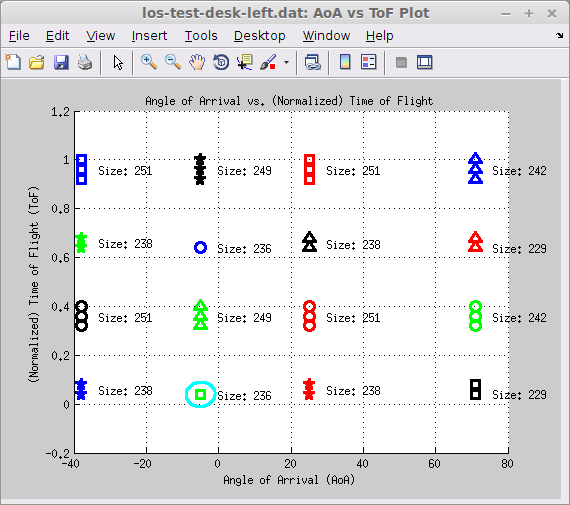
\includegraphics[width=0.4\textwidth]{../images/clustering-desk-left.png}
        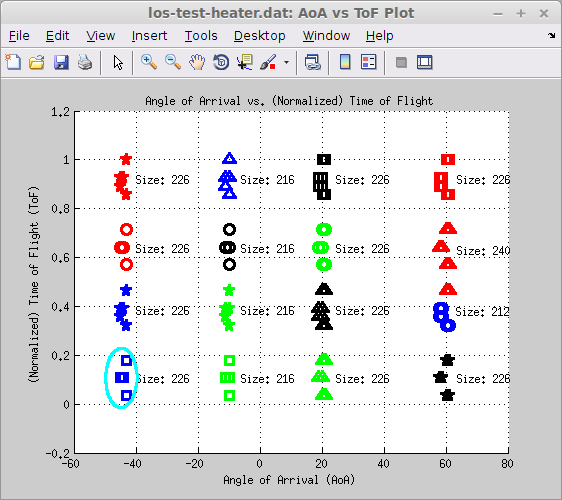
\includegraphics[width=0.4\textwidth]{../images/clustering-heater.png}
        \par\smallskip
        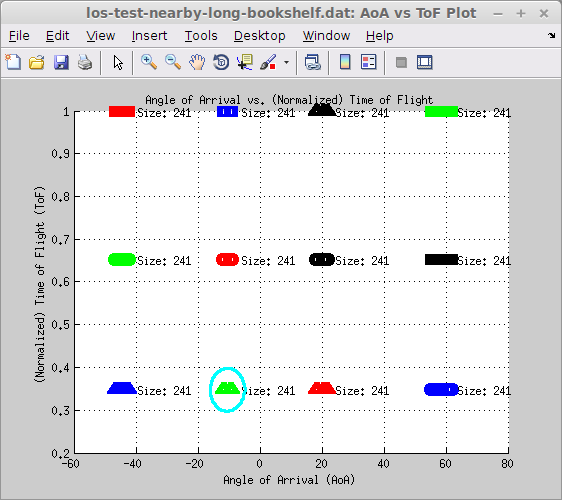
\includegraphics[width=0.4\textwidth]{../images/clustering-long-bookshelf.png}
        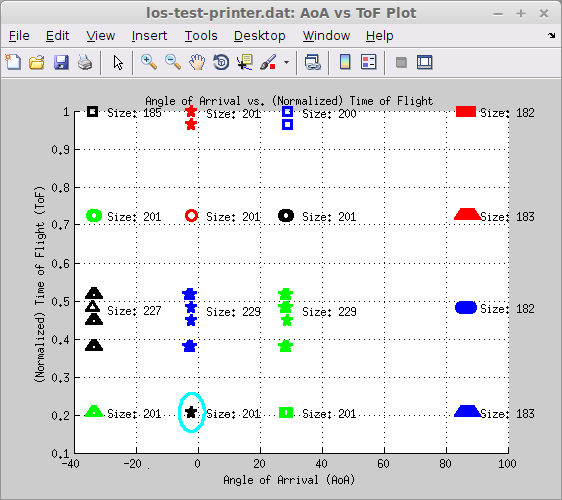
\includegraphics[width=0.4\textwidth]{../images/clustering-printer.png}
    \end{center}
\end{figure}

SpotFi runs the modified MUSIC algorithm for several packets and then clusters the results using each packet's computed normalized time of flight and normalized angle of arrival as two-dimensional coordinates. See figure \ref{figure: spotfi-clustering} for an example. The original SpotFi paper used Gaussian mean clustering to achieve this, which requires as input the expected number of clusters to generate, which equates to the number of multipath components. To make our implementation more robust to changing conditions, we used agglomerative clustering, which only takes qualitative cluster measurement parameters such as: the inner squared distance from point to cluster and the distance between the centers of clusters before the clusters are merged into one. These parameters can be easily determined prior to deployment. To determine these parameters I used collected channel state information from an ASUS 5 GHz router by pinging it when it was at several known locations. Afterwards I ran SpotFi on this data several times and tuned the clustering parameters until the clusters seemed correct. This tuning should hold across different deployments of LGTM since the time of flight and angle of arrival used in clustering are normalized. Therefore the distances are over normalized values which do not change. \par

A cluster is selected as the correct choice using a weighted likelihood computed using: number of points per cluster, average angle of arrival for the cluster, average time of flight for the cluster, and mean time of flight. 

$$w_{C} C_k - w_{\theta} \sigma_{\theta_{k}} - w_{\tau} \sigma_{\tau_{k}} - w_{s} \mu_{\tau_{k}}$$

Note that $C_k$ is the number of points in cluster $k$, $\sigma_{\theta_{k}}$ is the variance over the angle of arrival for cluster $k$, $\sigma_{\tau_{k}}$ is the variance over the time of flight for cluster $k$, and $\mu_{\tau_{k}}$ is the mean of the time of flight. The main idea behind this likelihood is that the cluster with the most points and the least variance (tightest clustering) should be selected since the direct signal path should have less variance in its measurements. The term with the mean time of flight for cluster $k$ is included since the signal with shorter time of flight should be more likely to be the direct path signal in line of sight scenarios. \par

To compute the weights for each of the likelihood terms, I used the collected channel state information from the ASUS 5 GHz router again and then fed cluster information labeled with the correct cluster choice into a linear support vector machine \cite{SvmTutorialBurges1998}. \par

% TODO: More detail on SVM?

The SpotFi system runs the modified version of MUSIC on multiple wireless access points and then combines the results from each to come up with a precise location. In my implementation, however, I am working from a single laptop, and so my implementation of SpotFi does no such combination, relying upon the angle of arrival computed on my single receiver. This certainly decreases the localization accuracy in comparison to the original SpotFi system; however, for this LGTM proof of concept, I think that is acceptable, especially since there has been very little work that can localize a wireless signal from a single point using commodity hardware. Furthermore, there are unique properties of LGTM that should mitigate localization errors. \par

I find myself working in a constrained scenario in comparison to the SpotFi paper however. SpotFi is a general wireless localization technique designed to work in non-line of sight and line of sight scenarios. In LGTM, there will always be a line of sight between the two users engaging in LGTM. Furthermore the distance between two users is expected to generally be quite small, and SpotFi's localization performs better over shorter distances \cite{SpotFiKotaru2015}. These constraints make me confident that this adapted SpotFi will be suitable enough for a proof of concept of LGTM. To validate this claim, I report localization accuracy results in the experiments section. \par

Since SpotFi is the most expensive operation in LGTM, I performed some optimizations to improve performance. In SpotFi, the angle of arrival is computed for each packet using the modified MUSIC algorithm, which is the most expensive part of the entire LGTM protocol. Since the packets are independent of one another, I parallelized the entire packet processing loop and improve the overall performance significantly. The processing speed is thus heavily linked to the number of cores used in processing. Adding additional cores will result in large speed ups. \par

I implement the modified SpotFi and MUSIC algorithm from scratch in MATLAB. To my knowledge there is no open-source implementation of SpotFi yet, despite apparently high demand \cite{SpotFiCsiToolIssue2016}, so I am releasing the source code for my SpotFi implementation and the entire LGTM protocol implementation. It is available at: \url{www.github.com/egaebel/lgtm}. \par

% TODO: Validation/testing on SpotFi

\subsection{Bringing It All Together}
The technologies described above are implemented in a combination of: C, C++, MATLAB, and Linux shell commands. To tie all this software together and construct a data pipeline for transmission, reception, processing, and user input, I use a Bash script to coordinate the flow of control. For passing state variables and data between separate programs, I use files for simplicity. The script first configures the wireless card to listen to the wireless channel for packets containing a special LGTM token and sets up a prompt for the user to initiate LGTM with a keystroke. When one user performs the keystroke on one of the testbed laptops a public key and random number are generated, concatenated together with an LGTM protocol string indicating it is the first message, and broadcast over the wireless channel. The LGTM protocol proceeds on autonomously as put forward in the protocol diagram in figure \ref{figure: protocol-diagram} with one important difference. Instead of sending a facial recognition model for each test device's assigned face, my implementation transmits a folder of images from the Yalefaces dataset, which is tarred (using the program tar) into an archive file. This folder contains a training set which is used by the recipient to train a facial recognition model. I found this method to be more efficient in terms of network usage since OpenCV's facial recognition models were very, very large. After both devices have received the images in the training set along with the channel state information associated with those packets, my modified version of SpotFi is run, and LGTM trains an LBPH facial recognition model using the training set. Now we have reached the human verification step. At this point, a window pops up displaying the real-time stream from the web cam attached to the laptop. Rendered atop the stream is a box around the recognized face (if there is one) and text below the box prompting the user to press space to confirm the face. See figure \ref{figure: lgtm-confirmation} If both users press space then LGTM is a success; otherwise, the two users may press escape to terminate LGTM. \par

\begin{figure}
    \begin{center}
        \caption{}
        \label{figure: lgtm-confirmation}
        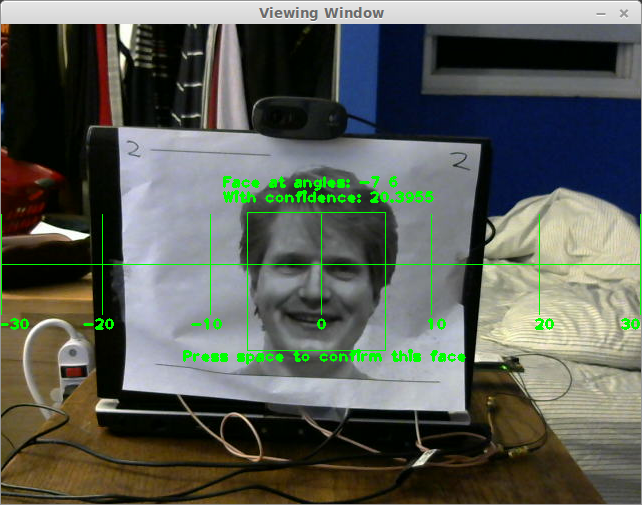
\includegraphics[scale=0.5]{../images/lgtm-confirmation.png}
    \end{center}
\end{figure}

% TODO: Conclusion for implementation

% Bash script for glue
% ---- File system usage
% ---- Linux tool usage
% ---- User input
% ---- Modularity
% ---- Ideal for debugging (file-by-file)

% Full System Walk-through
% ---- Data flow diagrams
% ---- Control flow diagrams
% ---- Walk-through (high level) of program execution with references to the components

\chapter{Experiments}
I found it prudent to run a few experiments to validate my implementation laid out in the previous section, particularly the wireless localization technique, as a sort of sanity check. In addition to validating the implementation, I also wanted to identify and validate potential performance enhancements since LGTM's core promise is usable security, and slow systems are less usable. My primary point of evaluation focuses on the performance and accuracy of the implementation of SpotFi adapted for point to point use since this is the most time consuming operation in LGTM, the primary component responsible for the security of this LGTM proof of concept, and my modifications are completely untested. \par

I also briefly discuss my validation of OpenCV's LBPH facial recognizer since it's being used in a non-traditional scenario. Most research in facial recognition deals with a known dataset of photos and feeds these photos directly into the facial recognition algorithms, often with some preprocessing first. LGTM trains on photos and tests on faces captured via web cam in real-time. This introduces additional noise since the faces are not perfectly centered in the x, y, or z axes and there is inherent noise in picking up a printed photo from a camera. For these reasons, it is fitting to briefly mention my evaluation methodology and mention the performance timing for training, if only to leave the reader without a doubt of the system's abilities. \par

\section{Wireless Localization -- SpotFi (FIX THIS TITLE HERE!! THIS ISN'T GREAT!)}

\begin{table}
    \begin{center}
        \caption{Base data results.}
        \label{table: base-data-table}
        \begin{tabular}{| c || c | c | c |}
\hline
Distances: & 1 m  & 2 m  & 3 m  \\
\hline
\hline
Correct in Top 1: & 47.0 \% & 27.0 \% & 24.0 \% \\
\hline
Correct in Top 2: & 77.0 \% & 41.0 \% & 36.0 \% \\
\hline
Correct in Top 3: & 90.0 \% & 66.0 \% & 48.0 \% \\
\hline
Correct in Top 4: & 100.0 \% & 74.0 \% & 49.0 \% \\
\hline
Correct in Top 5: & 100.0 \% & 74.0 \% & 49.0 \% \\
\hline
\hline
Mean Error: & 0.838 m & 1.543 m & 2.374 m \\
\hline
Median Error: & 0.803 m & 1.282 m & 2.368 m \\
\hline
\end{tabular}        
    \end{center}
\end{table}

\begin{table}
    \caption{Sampling data results.}
    \label{table: sampling-data-table}
    \begin{subfigure}[b]{0.3\textwidth}
        \begin{center}
            \scalebox{0.75}{\begin{tabular}{| c || c | c | c | c | c | c | c | c |}
\hline
Distance: &  &  &  & 1 m  &  &  &  &  \\
\hline
Number of Packets Used in SpotFi: & 1025 & 750 & 500 & 250 & 100 & 50 & 25 & 10 \\
\hline
\hline
Correct in Top 1: & 47.0 \% & 47.0 \% & 49.0 \% & 47.0 \% & 51.0 \% & 49.0 \% & 58.0 \% & 60.0 \% \\
\hline
Correct in Top 2: & 77.0 \% & 77.0 \% & 77.0 \% & 80.0 \% & 81.0 \% & 82.0 \% & 88.0 \% & 83.0 \% \\
\hline
Correct in Top 3: & 90.0 \% & 90.0 \% & 90.0 \% & 90.0 \% & 94.0 \% & 90.0 \% & 95.0 \% & 95.0 \% \\
\hline
Correct in Top 4: & 100.0 \% & 100.0 \% & 100.0 \% & 100.0 \% & 100.0 \% & 100.0 \% & 100.0 \% & 100.0 \% \\
\hline
Correct in Top 5: & 100.0 \% & 100.0 \% & 100.0 \% & 100.0 \% & 100.0 \% & 100.0 \% & 100.0 \% & 100.0 \% \\
\hline
\hline
Mean Error: & 0.838 m & 0.838 m & 0.829 m & 0.796 m & 0.768 m & 0.722 m & 0.790 m & 0.745 m \\
\hline
Median Error: & 0.803 m & 0.803 m & 0.789 m & 0.751 m & 0.703 m & 0.703 m & 0.757 m & 0.745 m \\
\hline
\end{tabular}}
        \end{center}
    \end{subfigure}
    \par\bigskip
    \begin{subfigure}[b]{0.3\textwidth}
        \begin{center}
            \scalebox{0.75}{\begin{tabular}{| c || c | c | c | c | c | c | c | c |}
\hline
Distance: &  &  &  & 2 m  &  &  &  &  \\
\hline
Number of Packets Used in SpotFi: & 1025 & 750 & 500 & 250 & 100 & 50 & 25 & 10 \\
\hline
\hline
Correct in Top 1: & 27.0 \% & 27.0 \% & 25.0 \% & 25.0 \% & 23.0 \% & 20.0 \% & 27.0 \% & 30.0 \% \\
\hline
Correct in Top 2: & 41.0 \% & 41.0 \% & 40.0 \% & 45.0 \% & 42.0 \% & 46.0 \% & 50.0 \% & 47.0 \% \\
\hline
Correct in Top 3: & 66.0 \% & 66.0 \% & 63.0 \% & 65.0 \% & 68.0 \% & 67.0 \% & 65.0 \% & 65.0 \% \\
\hline
Correct in Top 4: & 74.0 \% & 74.0 \% & 74.0 \% & 74.0 \% & 76.0 \% & 74.0 \% & 74.0 \% & 75.0 \% \\
\hline
Correct in Top 5: & 74.0 \% & 74.0 \% & 74.0 \% & 76.0 \% & 76.0 \% & 74.0 \% & 74.0 \% & 75.0 \% \\
\hline
\hline
Mean Error: & 1.543 m & 1.543 m & 1.487 m & 1.392 m & 1.565 m & 1.547 m & 1.484 m & 1.644 m \\
\hline
Median Error: & 1.282 m & 1.282 m & 1.213 m & 1.041 m & 1.278 m & 1.407 m & 1.233 m & 1.520 m \\
\hline
\end{tabular}}
        \end{center}
    \end{subfigure}
    \par\bigskip
    \begin{subfigure}[b]{0.3\textwidth}
        \begin{center}
            \scalebox{0.75}{\begin{tabular}{| c || c | c | c | c | c | c | c | c |}
\hline
Distance: &  &  &  & 3 m  &  &  &  &  \\
\hline
Number of Packets Used in SpotFi: & 1025 & 750 & 500 & 250 & 100 & 50 & 25 & 10 \\
\hline
\hline
Correct in Top 1: & 24.0 \% & 24.0 \% & 22.0 \% & 20.0 \% & 20.0 \% & 19.0 \% & 24.0 \% & 23.0 \% \\
\hline
Correct in Top 2: & 36.0 \% & 36.0 \% & 36.0 \% & 35.0 \% & 34.0 \% & 35.0 \% & 33.0 \% & 38.0 \% \\
\hline
Correct in Top 3: & 48.0 \% & 48.0 \% & 45.0 \% & 44.0 \% & 43.0 \% & 42.0 \% & 42.0 \% & 45.0 \% \\
\hline
Correct in Top 4: & 49.0 \% & 49.0 \% & 48.0 \% & 48.0 \% & 49.0 \% & 47.0 \% & 50.0 \% & 50.0 \% \\
\hline
Correct in Top 5: & 49.0 \% & 49.0 \% & 49.0 \% & 50.0 \% & 51.0 \% & 49.0 \% & 50.0 \% & 50.0 \% \\
\hline
\hline
Mean Error: & 2.374 m & 2.374 m & 2.405 m & 2.446 m & 2.444 m & 2.224 m & 2.477 m & 2.396 m \\
\hline
Median Error: & 2.368 m & 2.368 m & 2.289 m & 2.330 m & 2.367 m & 1.915 m & 2.739 m & 2.425 m \\
\hline
\end{tabular}}
        \end{center}
    \end{subfigure}
    \par\bigskip
\end{table}

\subsection{Accuracy}
Localization accuracy is front and center in LGTM. LGTM relies on wireless localization to provide guarantees about a transmitter's location, which is then used to bootstrap authentication. I found that my system performs modestly in comparison to other localization works, albeit not up to the high standards that a secure system would require. \par

To account for acceptable errors in angle of arrival computations, I introduce a slight error tolerance of 40 cm on either side of the face. Since I control the distance and angle between test devices in the experiment, I use the error tolerance and distance to compute the tolerance for the angle in degrees. \par

There are many lessons to gain from the data collected for LGTM's localization. LGTM uses a likelihood technique to make the final selection of angle of arrival. This can lead to an incorrect angle of arrival being selected over the correct one, sometimes by a very slim margin. To evaluate LGTM's localization accuracy with this in mind, I focus on the accuracy of the top-5 angle of arrival selections as well as the mean error and median error. Top-5, mean error, and median error accuracy reports for distances of: 1 meter, 2 meters, and 3 meters. The data used was gathered with the two testbed laptops at angles of: -20, -10, 0, 10, and 20 degrees, where 0 degrees is when the laptops are directly facing one another, +10 degrees indicates that one laptop is 10 degrees to the right of center and -10 degrees indicates that one laptop is 10 degrees left of center. The +/- 20 degree cases are the same as the +/- 10 degree cases. For each angle, I performed LGTM 10 times and saved off the channel state information used on each laptop. So this yields 20 samples for each angle at each distance and a total of 200 samples for each distance. \par 

The localization accuracy results are reported in table \ref{table: base-data-table}. As expected, localization accuracy is strongly coupled with the distance between devices. Percent correct in the top-1 position is almost halved when moving from 1 meter to 2 meters and beyond 2 meters the percent correct in the top-5 drops below 50\%. \par

\subsection{Performance}
Wireless localization performance is primarily bounded by the number of packets whose channel state information are used in computing the angle of arrival with the modified SpotFi implementation. As mentioned in the implementation section, I parallelize this since processing independent packets is an ``embarrassingly parallel'' problem. However, LGTM still incurs high performance penalties at this step due to the large number of packets. LGTM collects channel state information for the packets carrying the facial recognition parameters, which in this evaluation is actually just a tarred folder of photos which are used to train a facial recognition model. The number of packets to transmit this comes to approximately 1025 with minor variations due to slightly different image file sizes. Processing all these packets in the modified SpotFi takes up precious time, but using a large number of packets should intuitively provide better localization results. To examine the trade-off between localization accuracy and processing time I sampled different numbers of packets uniformly from the packet stream. Sampling sizes of 750, 500, 250, 100, 50, 25, and 10 were used. My findings are presented in table \ref{table: sampling-data-table} in comparison to the baseline localization results with no sampling. \par

Here I found something very surprising, reducing the number of packets increases localization accuracy. This could be explained by the presence of bursty noise which occurs in large chunks and throws off the clustering step in SpotFi, but this is simply speculation at this point. Regardless of what is causing this unexpected effect, I can certainly say that it is very positive. What I expected to be a trade-off between computation time and localization accuracy turned into an increase for both, a most pleasant surprise! \par

\section{Facial Recognition}
In deploying facial recognition in LGTM, I utilized the famous Yalefaces \cite{FisherfacesBelhumeur1997} dataset as a source of face photos. This dataset is not large, it includes photos of 15 subjects with 12 photos per subject. This should match the consumer use-case for LGTM quite well, since most users are not going to be willing to take many photos to train a facial recognition model. Most of each subject's set of photos contained one photo of the subject wearing glasses. A couple of subject's photo sets had the subject wearing glasses in all but a few photos. I removed from each subject's set of photos the least common eyewear choice. That is, if a subject was not wearing glasses in a majority of the photos, I removed the glasses photos, if the subject was mostly wearing glasses, I removed the photos without glasses. Recognizing users both with and without glasses makes facial recognition slightly more difficult, and in all LGTM use-cases, both users will need to be wearing augmented reality headsets, so keeping eye wear uniform makes sense for these experiments. \par

For evaluating facial recognition accuracy, I train on all images of one subject except one, the ``happy'' photo in each subject's set of photos. I then test recognition on this one omitted photo. Using this methodology, I was able to train an LBPH facial recognition model to accurately recognize every single subject in the Yalefaces dataset. \par

Facial recognition is not a performance bottleneck at all. I train a new classifier using the training photos on each run and it takes less than one second $[GET \: SOME \: REAL \: TIMES \: FOR \: THIS....they \: can \: be \: rough]$. Recognition itself is virtually instant; there is no noticeable lag time. \par

I can safely say, just from our cursory validation experiments on LBPH facial recognition for use-cases fitting LGTM that facial recognition is an efficient and accurate part of the whole LGTM system. \par


% TODO: Workshop this section or flat-out remove it
\section{Full System Timing (BETTER TITLE)}
Overall, my implementation of LGTM takes $<INSERT \: TIME \: TO \: RUN>$ seconds to run. On top of this, consider that there are various less than ideal procedures that I used to workaround various issues, and this timing is very good for a device pairing procedure. \par

\chapter{Conclusion}
\section{Future Work on LGTM}
There remains room to further improve LGTM by using more of the unique hardware and abilities that come with augmented reality. Simultaneous location and mapping (SLAM) is the field which explores mapping out a user's surroundings in terms of depth to objects and user location in the environment \cite{ParallelTrackingAndMappingKlein2007,MonoSlamDavison2007,VisualIntertialOdometryNonlinearLeutenegger2014,ProjectTangoWebsite,SlamPart1Durrant-Whyte2006}. No doubt many techniques from this field can be used to bolster LGTM's usability and make selecting users to share with even easier. \par

Of course, improved wireless localization accuracy will be a large contributor to improving LGTM. I fully expect the field to continue advancing the accuracy of wireless localization as it has over its entire existence. Indeed, since work on LGTM initially began, wireless localization has taken a huge step forward thanks to the works of Vasisht et al. in \cite{ChronosSingleAPLocalizationVasisht2016}, which describes a technique for performing decimeter level localization from a single access point with three antennas. \par

More work on analyzing LGTM itself also remains to be done. I have referenced a great many usability studies in this thesis, it would be great to perform one to get empirical data on LGTM's usability. \par

LGTM has been presented as a protocol to authenticate two users, but it can easily be expanded to include multiple users, however the exact method by which this should be done is not entirely clear. \par

Finally, a great deal of work can be done to examine augmented reality attacks in general, particularly ones involving spamming a users' vision or tricking users into accepting something inadvertently. There has been a small body of work on this topic already \cite{SafelyAugmentLebeck2016,SecurityAndPrivacyForARRoesner2014}, but for a new computational paradigm we are going to need a lot more. \par


\section{Conclusion}
 \par

%%%%%%%%%%%%%%%%%

%%%%%%%%%%%%%%%%%
%
% Include an EPS figure with this command:
%   \epsffile{filename.eps}
%

%%%%%%%%%%%%%%%%
%
% Do tables like this:

% \begin{table}
% \caption{The Graduate School wants captions above the tables.}
% \begin{center}
%  \begin{tabular}{ccc}
%  x & 1 & 2 \\ \hline
%  1 & 1 & 2 \\
%  2 & 2 & 4 \\ \hline
%  \end{tabular}
% \end{center}
% \end{table}

%%%%%%%%%%%%%%%%%%%%%%%%%%%%%%%%

% If you are using BibTeX, uncomment the following:
%\thebibliography
\bibliography{thesis-papers-db}
\bibliographystyle{IEEEtran}

%
% Otherwise, uncomment the following:
% \chapter*{Bibliography}

% \appendix

% In LaTeX, each appendix is a "chapter"
% \chapter{Program Source}

\end{document}